\documentclass{article}

% if you need to pass options to natbib, use, e.g.:
%     \PassOptionsToPackage{numbers, compress}{natbib}
% before loading neurips_2026

% The authors should use one of these tracks.
% Before accepting by the NeurIPS conference, select one of the options below.
% 0. "default" for submission
%\usepackage{neurips_2026}
\usepackage[eandd]{neurips_2026}
% the "default" option is equal to the "main" option, which is used for the Main Track with double-blind reviewing.
% 1. "main" option is used for the Main Track
%  \usepackage[main]{neurips_2026}
% 2. "position" option is used for the Position Paper Track
%  \usepackage[position]{neurips_2026}
% 3. "eandd" option is used for the Evaluations & Datasets Track
 % \usepackage[eandd]{neurips_2026}
 % if you need to opt-in for a single-blind submission in the E&D track:
 %\usepackage[eandd, nonanonymous]{neurips_2026}
% 4. "creativeai" option is used for the Creative AI Track
%  \usepackage[creativeai]{neurips_2026}
% 5. "sglblindworkshop" option is used for the Workshop with single-blind reviewing
 % \usepackage[sglblindworkshop]{neurips_2026}
% 6. "dblblindworkshop" option is used for the Workshop with double-blind reviewing
%  \usepackage[dblblindworkshop]{neurips_2026}

% After being accepted, the authors should add "final" behind the track to compile a camera-ready version.
% 1. Main Track
 % \usepackage[main, final]{neurips_2026}
% 2. Position Paper Track
%  \usepackage[position, final]{neurips_2026}
% 3. Evaluations & Datasets Track
 % \usepackage[eandd, final]{neurips_2026}
% 4. Creative AI Track
%  \usepackage[creativeai, final]{neurips_2026}
% 5. Workshop with single-blind reviewing
%  \usepackage[sglblindworkshop, final]{neurips_2026}
% 6. Workshop with double-blind reviewing
%  \usepackage[dblblindworkshop, final]{neurips_2026}
% Note. For the workshop paper template, both \title{} and \workshoptitle{} are required, with the former indicating the paper title shown in the title and the latter indicating the workshop title displayed in the footnote.
% For workshops (5., 6.), the authors should add the name of the workshop, "\workshoptitle" command is used to set the workshop title.
% \workshoptitle{WORKSHOP TITLE}

% "preprint" option is used for arXiv or other preprint submissions
 % \usepackage[preprint]{neurips_2026}

% to avoid loading the natbib package, add option nonatbib:
%    \usepackage[nonatbib]{neurips_2026}

\usepackage[utf8]{inputenc} % allow utf-8 input
\usepackage[T1]{fontenc}    % use 8-bit T1 fonts
\usepackage{hyperref}       % hyperlinks
\usepackage{url}            % simple URL typesetting
\usepackage{booktabs}       % professional-quality tables
\usepackage{amsfonts}       % blackboard math symbols
\usepackage{nicefrac}       % compact symbols for 1/2, etc.
\usepackage{microtype}      % microtypography
\usepackage{xcolor}         % colors
\usepackage{amsmath,amssymb,amsfonts,amsthm}
\newtheorem{definition}{Definition}
\usepackage{graphicx}
\usepackage{subcaption} % in preamble
\usepackage[table]{xcolor}

% ── TikZ (required for architecture diagram in appendix) ────────────────────
\usepackage{tikz}
\usetikzlibrary{positioning, arrows.meta, shapes.geometric, calc}

% ── Colors used in architecture diagram ─────────────────────────────────────
\definecolor{memteal}{RGB}{26,188,156}
\definecolor{mempurple}{RGB}{142,68,173}
\definecolor{memred}{RGB}{192,57,43}

% ── Figures are stored in new-figs/ relative to this .tex file ───────────────
\graphicspath{{new-figs/}}

% Note. For the workshop paper template, both \title{} and \workshoptitle{} are required, with the former indicating the paper title shown in the title and the latter indicating the workshop title displayed in the footnote.
\newcommand{\memeic}{\textbf{MemEIC}}

\title{CCKEB and Adversarial-2k: Benchmarks for Compositional and Adversarial Multimodal Knowledge Editing}


% The \author macro works with any number of authors. There are two commands
% used to separate the names and addresses of multiple authors: \And and \AND.
%
% Using \And between authors leaves it to LaTeX to determine where to break the
% lines. Using \AND forces a line break at that point. So, if LaTeX puts 3 of 4
% authors names on the first line, and the last on the second line, try using
% \AND instead of \And before the third author name.


\author{%
  Anonymous Author(s)\thanks{Submitted to NeurIPS 2026 Evaluations \& Datasets Track.} \\
  Under Double-Blind Review\\
}


\begin{document}


\maketitle


\begin{abstract}
We introduce two complementary benchmarks for evaluating multimodal knowledge editing. \textbf{CCKEB} (Compositional Continual Knowledge Editing Benchmark) provides 6{,}278 image--text pairs (5{,}000 train / 1{,}278 eval) for continual compositional editing, covering diverse entities and structured relational knowledge. \textbf{Adversarial-2k} is a held-out stress-test of 2{,}000 samples balanced across five cross-modal failure modes: Polysemy (F1), Cross-Modal Conflict (F2), Near-Miss Retrieval (F3), Multi-Hop Reasoning (F4), and Hard Visual Distinction (F5), with 400 samples per category. Each sample includes a visual edit, a textual edit, a compositional query, a ground-truth answer, a rephrased query variant, portability probes, and locality checks. Constructed through a failure-guided pipeline with adversarial filtering (64\% acceptance rate), the datasets expose systematic weaknesses invisible to standard benchmarks. Evaluation of six editing methods reveals that Cross-Modal Conflict remains effectively unsolved ($<$10.5\% EA for all methods) and that compositional reliability lags edit accuracy by 20--24 percentage points across the board. Both datasets, code, and evaluation scripts are released publicly to support reproducible research.
\end{abstract}



\section{Introduction}
\label{sec:intro}


Knowledge editing aims to update specific facts in a model without full retraining, enabling targeted modifications while preserving existing behavior \cite{editing23,easyedit24,KE_24survey}. While this problem has been widely studied in language-only models, extending it to large vision--language models (LVLMs) \cite{BLIP-2_2023,minigpt24} introduces new challenges. In LVLMs, knowledge is distributed across visual and textual modalities, and edits must remain consistent across both while supporting compositional reasoning over multiple updates. Existing benchmarks have begun to evaluate these capabilities under compositional and continual editing settings, but they primarily assess performance under clean or standard conditions. As a result, current evaluations do not reveal whether multimodal knowledge editing systems remain robust under adversarial cross-modal failures such as ambiguity, conflicting signals, and near-miss evidence.


\par For example, answering ``What is the title of the person in this image?'' after updating both identity and role requires combining visual identity with updated textual attributes. Standard compositional editing benchmarks test this capability, but they do not explicitly isolate failure cases where cross-modal fusion is stressed by ambiguity, conflicting evidence, or near-miss retrieval. Recent approaches, such as memory-augmented editors (e.g., MemEIC), improve multimodal editing through fusion and external knowledge. However, when evaluated under adversarial cross-modal conditions, even strong models exhibit consistent failure patterns involving semantic ambiguity, modality conflicts, and multi-step reasoning. These failures highlight a gap in current evaluation protocols, which remain insufficient to diagnose when and why multimodal knowledge editing breaks down.

\par We argue that existing benchmarks fail not because models cannot edit knowledge under continual and compositional settings, but because they do not systematically stress-test cross-modal reasoning under controlled adversarial failure scenarios. To address this gap, we introduce Adversarial-2k, a held-out adversarial benchmark for multimodal knowledge editing. Adversarial-2k constructs controlled examples across semantic ambiguity, near-miss visual similarity, modality conflicts, and multi-hop compositional queries. These scenarios test whether models trained or edited under standard continual-compositional settings can generalize to challenging cross-modal conditions. We evaluate existing knowledge editing approaches on Adversarial-2k and observe consistent performance degradation, particularly in cases requiring cross-modal consistency and compositional reasoning. This shows that current models struggle to maintain coherent updates when knowledge must propagate across modalities.


\par \textbf{Contributions} We make four main contributions: (1) we introduce Adversarial-2k, a held-out adversarial benchmark for multimodal knowledge editing that systematically stress-tests models under controlled conditions such as semantic ambiguity, modality conflicts, near-miss visual similarity, and multi-hop compositional queries, with examples balanced across these failure modes; (2) we identify and formalize five systematic failure modes in multimodal knowledge editing, providing a structured taxonomy of cross-modal composition errors; (3) we evaluate existing knowledge editing methods trained or edited under standard continual-compositional settings on Adversarial-2k and reveal consistent performance degradation across failure categories; and (4) we provide diagnostic insights into these failures, exposing limitations in current cross-modal fusion and knowledge propagation mechanisms.


% Knowledge editing aims to update specific facts in a model without full retraining, enabling targeted modifications while preserving existing behavior \cite{editing23,easyedit24,KE_24survey}. While this problem has been widely studied in language-only models, extending it to large vision–language models (LVLMs) \cite{BLIP-2_2023,minigpt24} introduces new challenges. In LVLMs, knowledge is distributed across visual and textual modalities, and edits must remain consistent across both while supporting compositional reasoning over multiple updates. However, existing benchmarks largely evaluate knowledge editing under simplified, atomic settings, where edits are independent and unambiguous. These assumptions break down in multimodal scenarios, where ambiguity, conflicting signals, and cross-modal dependencies are common. As a result, current evaluations miss the core difficulty of multimodal knowledge editing, leaving critical failure cases untested.

% \par For example, answering ``What is the title of the person in this image?'' after updating both identity and role requires combining visual identity with updated textual attributes. Existing benchmarks fail to expose systematic weaknesses in cross-modal fusion mechanisms, which are central to large vision--language models. Recent approaches, such as memory-augmented editors (e.g., MemEIC), attempt to address multimodal editing through improved fusion and external knowledge. However, even strong models exhibit consistent failure patterns under challenging conditions, including semantic ambiguity, modality conflicts, and multi-step reasoning. These failures highlight a fundamental gap in current evaluation protocols, which remain insufficient to diagnose how and why multimodal knowledge editing breaks down.


% 


% \par \textbf{Contributions} We make four main contributions: (1) we introduce Adversarial-2k, a new benchmark for multimodal knowledge editing that systematically stress-tests models under controlled conditions such as semantic ambiguity, modality conflicts, near-miss visual similarity, and multi-hop compositional queries, with examples balanced across these failure modes; (2) we identify and formalize five systematic failure modes in multimodal knowledge editing, derived from empirical analysis, providing a structured taxonomy of cross-modal composition errors; (3) we evaluate existing knowledge editing methods on Adversarial-2k and reveal consistent performance degradation and significant gaps across failure categories; and (4) we provide diagnostic insights into these failures, exposing fundamental limitations in current cross-modal fusion and knowledge propagation mechanisms.

% \begin{figure}[t]
%   \centering
%   \includegraphics[width=\linewidth]{new-figs/fig3_dataset_comparison.png}
%   \caption{%
%     \textbf{Comparison with existing multimodal knowledge-editing datasets.}
%     Bars indicate whether each dataset supports key evaluation properties:
%     compositional QA, continual editing, adversarial stress-testing, and
%     multi-model evaluation. The line shows dataset size on the right axis.
%     Adversarial-2k complements prior benchmarks by adding controlled
%     adversarial stress tests for cross-modal reasoning.
%   }
%   \label{fig:comparison}
% \end{figure}




\begin{figure*}[t]
  \centering
  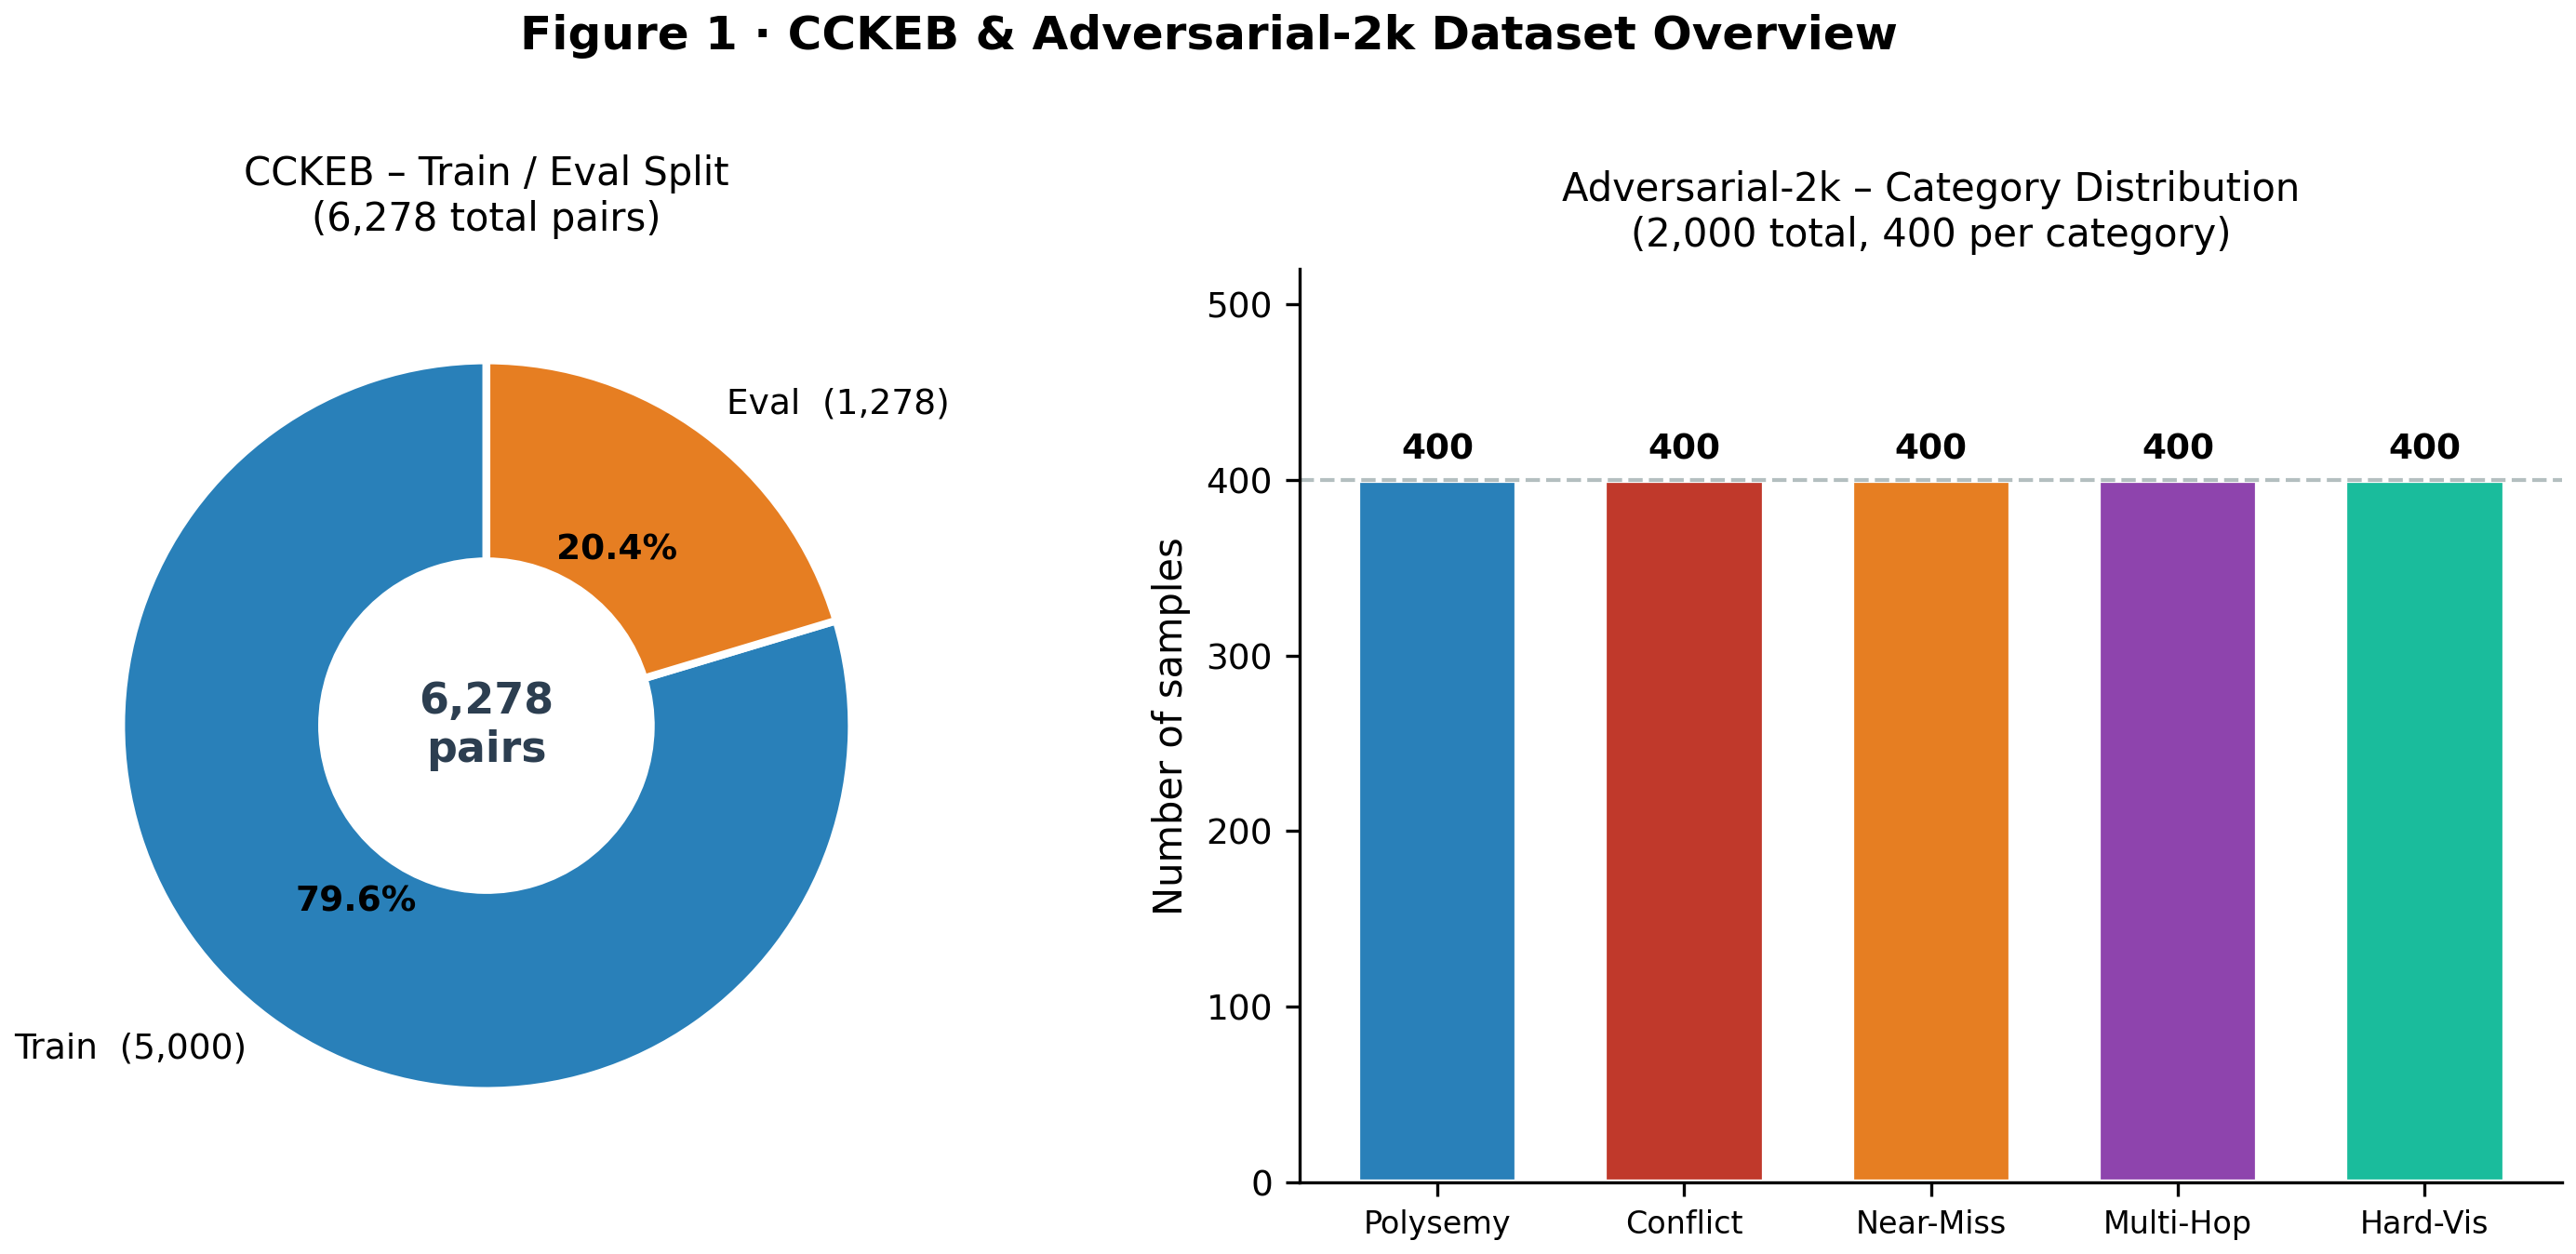
\includegraphics[width=\linewidth]{fig1_dataset_overview.png}
  \caption{%
    \textbf{Overview of the CCKEB and Adversarial-2k datasets.}
    \emph{Left:} CCKEB train/eval split: 6{,}278 total pairs distributed as
    5{,}000 training pairs (79.6\%) and 1{,}278 evaluation pairs (20.4\%),
    providing the continual-compositional editing benchmark used to train and
    evaluate editing methods.
    \emph{Right:} Category distribution of Adversarial-2k: 2{,}000 samples
    evenly split across five failure modes (400 per category: Polysemy,
    Cross-Modal Conflict, Near-Miss Retrieval, Multi-Hop Reasoning, and Hard
    Visual Distinction), confirming balanced coverage of all adversarial
    scenarios.
    Together these panels establish the scale and balance of the two datasets
    introduced in this work.
  }
  \label{fig:dataset_overview}
\end{figure*}

\section{Related Work}

\paragraph{Knowledge editing in language models.}
Knowledge editing has attracted significant attention as a practical alternative to full model retraining for updating specific factual associations in large language models~\cite{editing23,KE_24survey,easyedit24}. Locate-and-edit methods such as ROME~\cite{rome22} and MEMIT~\cite{memit23} identify causally relevant weight layers via causal tracing and perform rank-one or rank-$k$ updates confined to those locations, enabling precise factual edits with minimal side effects. MEND~\cite{mend22} takes a meta-learning approach, training a hypernetwork that converts task gradients into low-rank parameter updates and achieving fast adaptation at scale without storing explicit memory. Retrieval-based approaches offer a complementary mechanism: SERAC~\cite{serac22} routes queries through a learned scope classifier and answers in-scope queries using a counterfactual model, while IKE~\cite{ike23} treats in-context demonstrations of edited facts as a parameter-free alternative that avoids any weight modification. WISE~\cite{wise24} introduces a dual-memory architecture that separates edited knowledge into dedicated side memories, enabling lifelong editing without catastrophic forgetting. Despite this diversity of mechanisms, the benchmarks used to evaluate these methods---ZsRE, CounterFact, and their derivatives---are designed for single, atomic, text-only edits and do not test whether edited knowledge can be composed across modalities or propagated through multi-step reasoning chains. This evaluation gap is precisely what motivates the datasets we introduce.

\paragraph{Continual and sequential knowledge editing.}
A growing body of work recognises that real-world deployment requires models to absorb long sequences of updates rather than isolated edits~\cite{KE_24survey}. Sequential editing poses two compounding difficulties: \emph{accumulation}, where each new edit increases the risk of interfering with prior updates, and \emph{propagation}, where later edits may invalidate facts derived from earlier ones. GRACE~\cite{wise24} addresses accumulation through codebook-based side memories that expand with each edit, preventing weight interference at the cost of retrieval overhead. ContinualEdit~\cite{easyedit24} studies interference across hundreds of sequential edits and demonstrates that locate-and-edit methods degrade sharply beyond a few dozen updates. In the continual setting, evaluation protocols must therefore track not only whether individual edits succeed, but whether previously edited facts remain intact (locality) and whether dependent facts are updated consistently (portability). The Compositional Continual Knowledge Editing Benchmark (CCKEB) introduced alongside Adversarial-2k directly targets this setting, providing 5{,}000 training pairs and 1{,}278 evaluation pairs designed to stress-test both accumulation robustness and cross-edit compositional consistency. Adversarial-2k complements CCKEB by evaluating whether models that have been trained or evaluated under continual-compositional conditions can further withstand adversarially constructed cross-modal queries.

\paragraph{Evaluation datasets for knowledge editing.}
The development of rigorous evaluation datasets has been a bottleneck for the field. Early benchmarks such as ZsRE~\cite{editing23} and CounterFact~\cite{rome22} provide isolated text-only fact edits but lack systematic coverage of multi-hop dependencies, paraphrase robustness, or locality constraints. T-REx and TriviaQA have been repurposed for editing evaluation but suffer from label ambiguity under counterfactual conditions. RIPPLEEDITS~\cite{KE_24survey} takes a structured approach, measuring how a single edit ripples through dependent facts, and reveals that even strong editors propagate changes to only a fraction of logically downstream queries. MQUAKE~\cite{easyedit24} specifically targets multi-hop compositional queries constructed from Wikidata reasoning chains, showing that current editors fail badly when the correct answer requires chaining two or more updated facts. In the multimodal space, VLKEB~\cite{vlkeb24} provided the first large-scale visual-language editing benchmark, while MIKE~\cite{mike24} introduced fine-grained edit types covering visual entity, attribute, and relation updates. A critical limitation shared by all these datasets is that evaluation dimensions---edit accuracy, rephrase accuracy, portability, and locality---are measured independently rather than jointly under adversarial compositional pressure. Adversarial-2k is the first evaluation dataset to combine controlled adversarial construction, failure-mode stratification, and balanced compositional coverage, and to apply this framework specifically to multimodal knowledge editing.

\paragraph{Multimodal knowledge editing and vision--language models.}
Extending knowledge editing to large vision--language models (LVLMs)~\cite{BLIP-2_2023,minigpt24} introduces cross-modal dependencies that text-only methods do not address. In LVLMs, a single fact may be expressed through visual grounding, textual attributes, or both simultaneously, and an edit must remain consistent across all such representations. MLLM-Edit~\cite{mllmedit23} focuses on correcting hallucinations in multimodal large language models by patching the language head, but does not address visual-side edits or cross-modal consistency. VLKEB~\cite{vlkeb24} provides 2{,}400 entity-centric image--text pairs for visual-language editing but evaluates visual and textual edits independently, leaving the compositional interaction unprobed. MIKE~\cite{mike24} decomposes edits into three types---visual entity, visual attribute, and textual relation---but treats them as separate evaluation tracks rather than requiring joint reasoning across tracks. \memeic{}~\cite{memeic2025} proposes dual external memory with separate visual and textual streams fused through a brain-inspired gated connector, establishing a strong baseline for compositional multimodal editing. In our evaluation, we treat \memeic{} as the primary evaluated system and show that even this strong baseline degrades substantially under the adversarial cross-modal conditions captured by Adversarial-2k, particularly in the Cross-Modal Conflict category (0.8\% EA) where visual evidence directly contradicts the edited textual knowledge.

\paragraph{Compositional evaluation benchmarks in vision--language models.}
Compositional evaluation of pre-trained vision--language models has independently motivated a rich line of diagnostics. WinoGround~\cite{winoground22} demonstrates that state-of-the-art contrastive models fail to distinguish images paired with compositionally similar captions that differ only in word order, revealing an insensitivity to structural binding. ARO~\cite{aro23} shows that CLIP-style models function effectively as bags-of-words, failing attribute-binding and relation-binding probes despite high aggregate accuracy. GQA~\cite{gqa19} provides structured scene-graph-grounded multi-step questions, while OK-VQA~\cite{okvqa19} requires external knowledge beyond the image for correct answers. These benchmarks establish that compositional and knowledge-intensive reasoning remain unsolved challenges in pre-trained models; our work asks a strictly harder question---whether these challenges become more acute after knowledge editing, when the model's representations are modified and the correct answer depends on reasoning jointly over a visual input and a recently injected textual fact. Adversarial VQA~\cite{li2019vqa} further demonstrates that even carefully controlled benchmarks can be solved by exploiting dataset biases rather than visual reasoning; our adversarial filtering pipeline (64\% acceptance rate) is designed to prevent the same shortcut paths from appearing in Adversarial-2k.

\paragraph{Dataset construction methodology and quality standards.}
Dataset quality in evaluation benchmarks is as important as coverage, and recent work has highlighted failure modes in dataset construction that introduce spurious correlations, annotation artifacts, and train--test contamination~\cite{gqa19,okvqa19}. For knowledge-editing benchmarks specifically, a critical issue is \emph{trivial solvability}: samples that can be answered from a single modality or from surface-level cues without applying the edit. CounterFact~\cite{rome22} addresses this by using subject-relation-object triples where the counterfactual object is implausible but grammatically valid; MQUAKE~\cite{easyedit24} enforces multi-hop necessity by constructing chains where no single hop suffices. Adversarial-2k extends this quality philosophy to the multimodal compositional setting. Each candidate sample must pass four annotation criteria---bimodal necessity, answer uniqueness, visual grounding clarity, and failure-category attribution---validated by three independent annotators. Rejected samples are replaced rather than corrected, and inter-annotator agreement is monitored to avoid category drift. This rigorous protocol, combined with the failure-guided construction strategy (Section~\ref{sec:dataset_construction}), ensures that Adversarial-2k measures genuine compositional reasoning rather than dataset-specific shortcuts, and positions it as a reliable diagnostic tool for the evaluation of multimodal knowledge editing systems.

Figure~\ref{fig:comparison} situates Adversarial-2k and CCKEB within the landscape of existing multimodal knowledge-editing datasets across four key properties. No prior dataset simultaneously supports compositional query evaluation, continual editing, adversarial stress-testing, and multi-model evaluation. Adversarial-2k is the only benchmark providing systematic adversarial stress-tests; CCKEB is the only one combining compositional and continual editing support. Together, the two datasets fill a gap that has left the community without reliable tools to diagnose where and why multimodal knowledge editing fails under realistic, challenging conditions.

\begin{figure}[t]
  \centering
  \includegraphics[width=\linewidth]{fig3_dataset_comparison.png}
  \caption{%
    \textbf{CCKEB and Adversarial-2k vs.\ existing multimodal knowledge-editing datasets.}
    Bars indicate whether each dataset supports the property (\checkmark = yes,
    $\times$ = no) across four dimensions: compositional QA, continual editing
    support, adversarial stress-testing, and multi-model evaluation.
    The dashed line (right axis) shows dataset size in thousands of samples.
    CCKEB (Ours) is the only benchmark combining compositional and continual
    editing support; Adversarial-2k (Ours) is the only one providing systematic
    adversarial stress-testing. No prior dataset achieves all four properties
    simultaneously.
  }
  \label{fig:comparison}
\end{figure}


\section{Adversarial-2k Dataset}

\subsection{Task Definition}
\label{sec:problem}

We consider the task of multimodal compositional knowledge editing, where a model must incorporate edits across visual and textual modalities and answer queries conditioned on both.

\begin{definition}[Multimodal Knowledge Edit]
A \emph{multimodal knowledge edit} consists of a tuple $(I, e, e', r, o, o')$, where $I$ is an image containing entity $e$; $(e, r, o)$ is a source fact triplet; $e' \neq e$ is the target entity identity (visual edit); and $o' \neq o$ is the target object value (textual edit). After applying the edit, the model is required to answer queries such as ``What is the $r$ of the person in this image?'' with answer $o'$.
\end{definition}


\subsection{Cross-Modal Composition Failure Taxonomy}
\label{sec:taxonomy}

We define five cross-modal composition failure categories that structure the Adversarial-2k dataset. Each category captures a distinct challenge in multimodal compositional reasoning and is used to guide both dataset construction and evaluation. Table~\ref{tab:taxonomy} summarises these categories along with their underlying type and root cause.

\begin{table}[t]
\centering
\caption{Cross-modal composition failure taxonomy. Each category captures a distinct challenge in multimodal compositional reasoning.}
\label{tab:taxonomy}
\small
\begin{tabular}{@{}llcl@{}}
\toprule
\textbf{F\#} & \textbf{Failure Mode} & \textbf{Category} & \textbf{Root Cause} \\
\midrule
F1 & Polysemy              & Retrieval & Visual entity maps to multiple textual meanings \\
F2 & Cross-Modal Conflict  & Fusion    & Visual evidence contradicts edited textual knowledge \\
F3 & Retrieval Error       & Retrieval & Incorrect or near-miss memory retrieved \\
F4 & Reasoning Chain       & Inference & Failure in multi-step compositional reasoning \\
F5 & Hard Visual Dist.     & Visual    & Confusion between visually similar entities \\
\bottomrule
\end{tabular}
\end{table}

\textbf{Polysemy (F1)} arises when a visual entity admits multiple valid textual interpretations, introducing ambiguity during retrieval. 
\textbf{Cross-Modal Conflict (F2)} occurs when visual evidence contradicts the edited textual knowledge, requiring the model to resolve conflicting signals across modalities. 
\textbf{Retrieval Error (F3)} corresponds to near-miss memory retrieval, where semantically similar but incorrect facts are selected. 
\textbf{Reasoning Chain (F4)} captures failures in multi-step inference over updated knowledge, where dependencies across reasoning steps are not correctly maintained. 
\textbf{Hard Visual Distinction (F5)} reflects confusion between visually similar yet semantically distinct entities, leading to incorrect grounding.

Figure~\ref{fig:taxonomy} provides a quantitative view of the five failure modes, showing both the frequency of each mode in the 195-error audit (blue) and its average annotator-rated severity on a 0--5 scale (red). Cross-Modal Conflict is the most severe despite moderate frequency, while Polysemy is the most frequent but comparatively more tractable.

\begin{figure}[t]
  \centering
  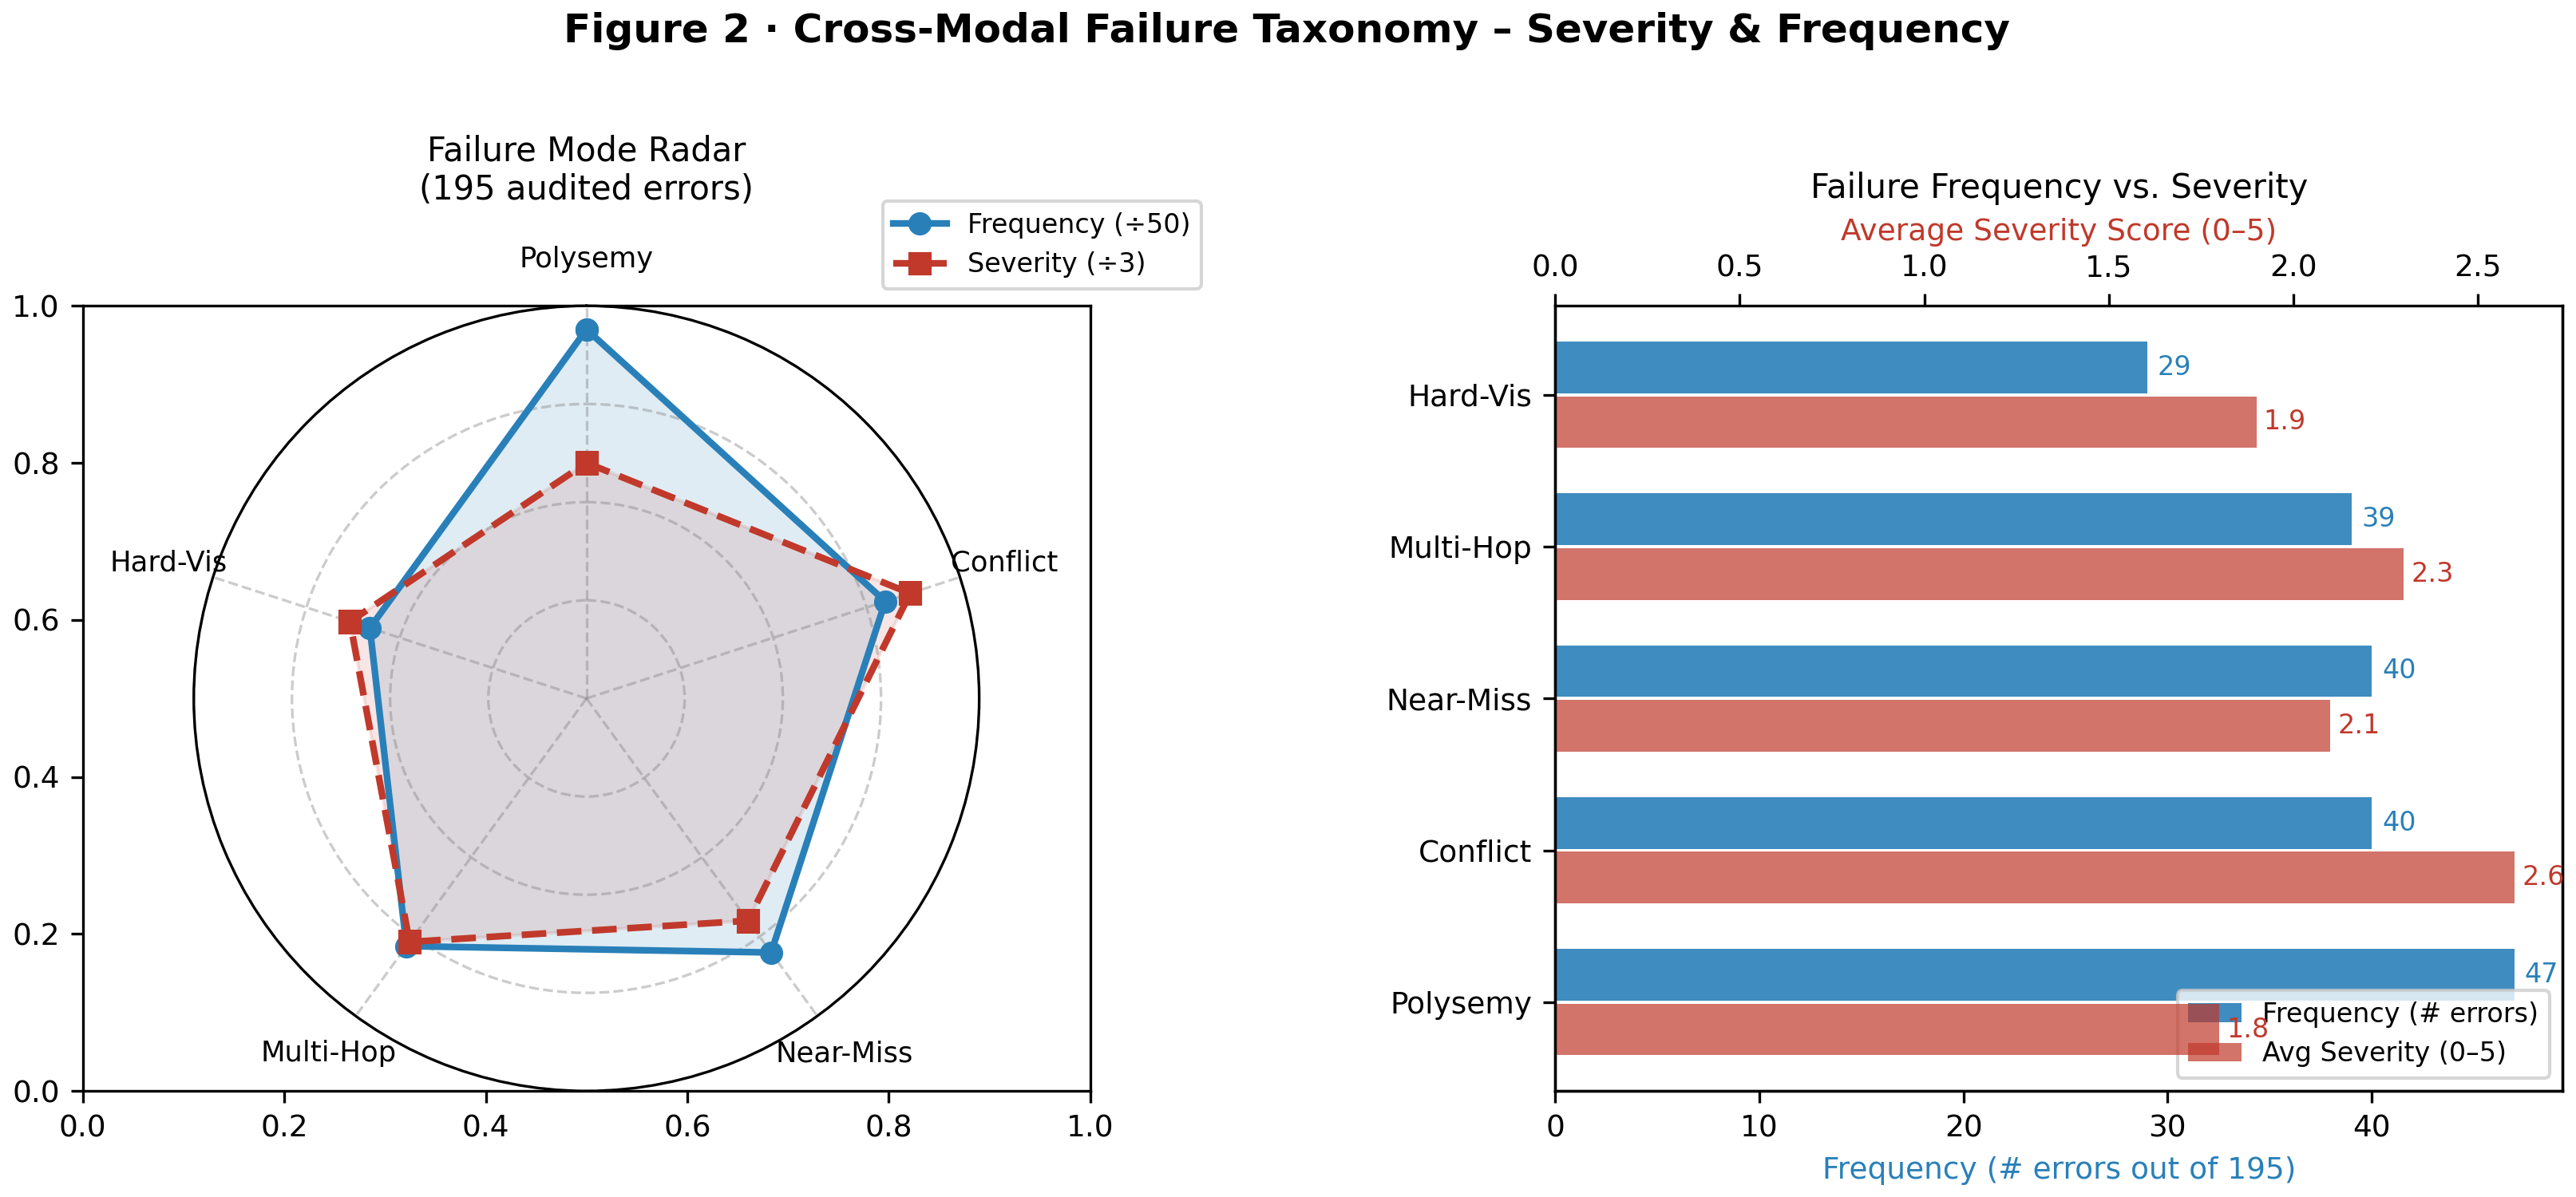
\includegraphics[width=\linewidth]{fig2_failure_taxonomy.png}
  \caption{%
    \textbf{Failure taxonomy: frequency vs.\ severity.}
    \textit{Left}: Radar chart showing normalised frequency (blue) and
    severity score (red) for each failure mode derived from a 195-error audit.
    \textit{Right}: Absolute counts and average severity.
    Cross-Modal Conflict (F2) is the most severe; Polysemy (F1) is the most
    frequent. Both dimensions inform dataset construction priorities.
  }
  \label{fig:taxonomy}
\end{figure}


\subsection{Dataset Construction}
\label{sec:dataset_construction}

Adversarial-2k is constructed to systematically capture multimodal compositional editing under controlled failure scenarios. The dataset is designed around three core principles: \textbf{compositionality}, \textbf{adversarial targeting}, and \textbf{categorical balance}. Each sample requires jointly reasoning over both visual and textual edits, ensuring that the correct answer cannot be derived from a single modality alone. Samples are explicitly constructed to target the failure categories defined in Section~\ref{sec:taxonomy}, enabling coverage of challenging compositional scenarios. In addition, the dataset is balanced across categories, with 2{,}000 samples evenly distributed (400 per category), ensuring fair evaluation.

\textbf{Failure-guided design.}
The dataset is generated in a failure-guided manner, where the predefined taxonomy directly informs sample construction. This approach ensures systematic coverage of diverse compositional settings while maintaining consistency across categories.

\textbf{Construction pipeline.}
The dataset is constructed through five stages. \textbf{(1) Source data selection:} Images are sampled from the COCO Train2017 split to provide naturalistic visual inputs, while textual knowledge is derived from structured relational triples spanning domains such as professions, nationalities, and biological categories. \textbf{(2) Visual edit generation:} A visual edit $(I, e, e')$ is defined for each sample, where the target identity $e'$ is selected according to the intended failure category. \textbf{(3) Textual edit generation:} A corresponding textual edit $(e', r, o, o')$ is generated by modifying the object value associated with relation $r$, with multi-hop relational chains introduced for reasoning-intensive scenarios. \textbf{(4) Query construction:} A natural language query $q$ is constructed such that answering it requires both identifying $e'$ from the image and retrieving $o'$ via relation $r$; a paraphrased variant is also included to reduce surface-form bias. \textbf{(5) Adversarial filtering:} Candidate samples are refined to ensure alignment with the intended failure category and to enforce compositional difficulty. Samples that can be solved using a single modality or admit ambiguous answers are discarded, resulting in an acceptance rate of approximately 64\%.

Figure~\ref{fig:pipeline} illustrates all five construction stages and how each feeds into the final Adversarial-2k dataset.

\begin{figure}[t]
  \centering
  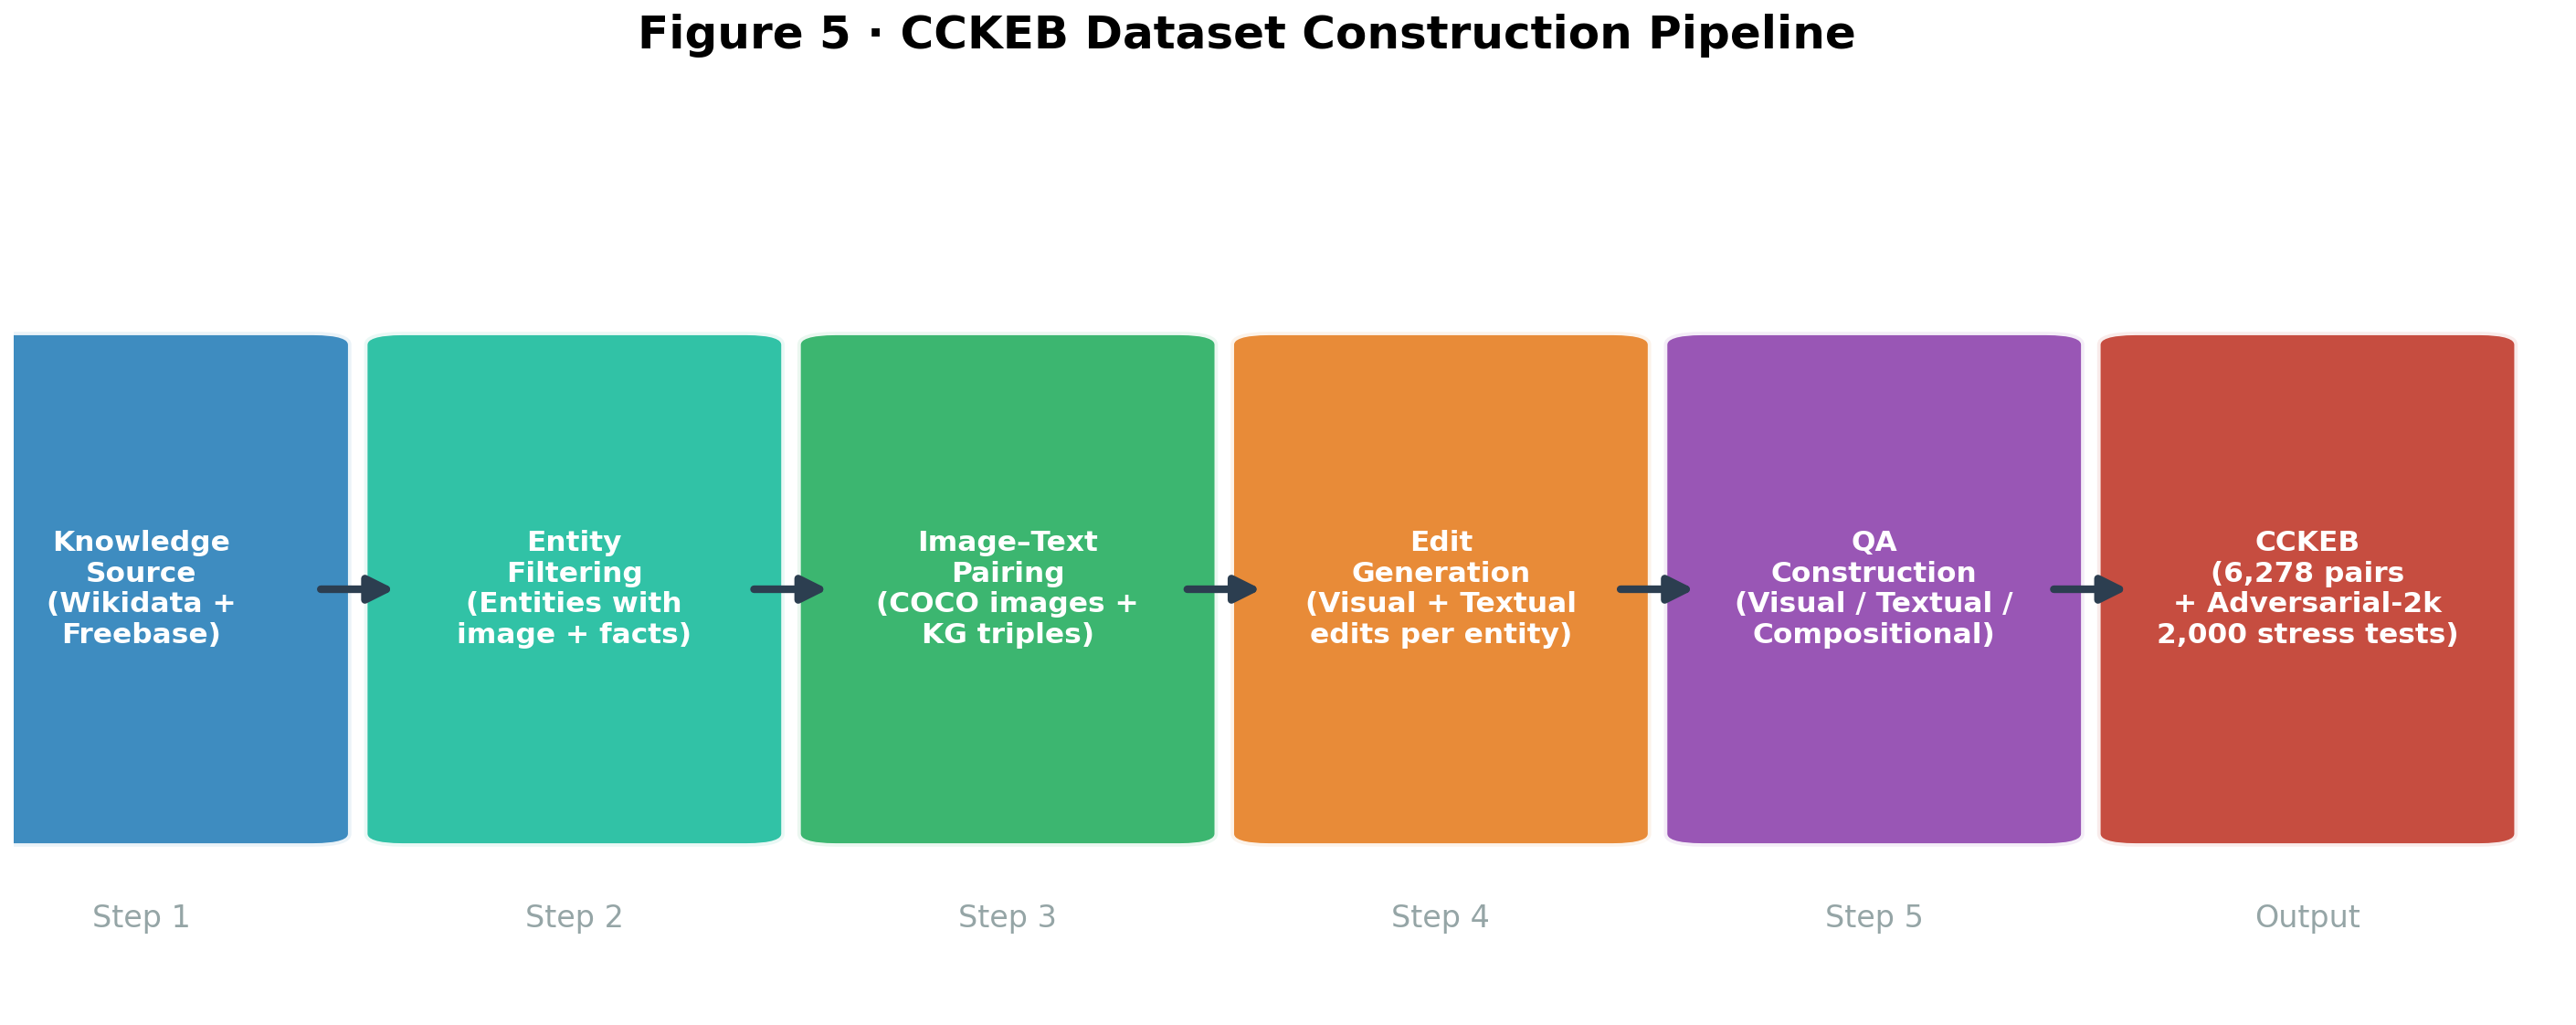
\includegraphics[width=\linewidth]{fig5_construction_pipeline.png}
  \caption{%
    \textbf{Five-stage construction pipeline for CCKEB and Adversarial-2k.}
    Stage~1: entity-centric knowledge is sourced from Wikidata and Freebase.
    Stage~2: entities are filtered to those with both associated images and
    structured relational facts.
    Stage~3: filtered entities are paired with COCO images and knowledge-graph
    triples to form image--text instances.
    Stage~4: visual and textual edits are generated for each entity pair.
    Stage~5: compositional QA probes (visual, textual, and compositional
    variants) are constructed.
    The final output is CCKEB (6{,}278 pairs) together with the 2{,}000
    Adversarial-2k stress-test samples derived from the same pipeline with an
    additional adversarial filtering pass ($\approx$64\% acceptance rate).
  }
  \label{fig:pipeline}
\end{figure}


% ─────────────────────────────────────────────────────────────
\subsection{Annotation and Quality Control}

\textbf{Annotation protocol.}
Each sample is validated by three independent annotators under four criteria: \textbf{(1) bimodal necessity}, ensuring that the answer cannot be inferred from a single modality; \textbf{(2) answer uniqueness}, requiring a single correct answer; \textbf{(3) visual grounding}, verifying that the entity is clearly identifiable in the image; and \textbf{(4) failure attribution}, ensuring that each sample corresponds to a well-defined failure category. Samples failing any criterion are removed and replaced.

\textbf{Quality control.}
Rejected samples are replaced rather than corrected. Inter-annotator agreement is monitored, and ambiguous cases are resolved through majority review. A final validation step ensures balanced representation across categories and prevents trivial shortcuts.


\subsection{Dataset Statistics}
Adversarial-2k consists of 2{,}000 samples evenly distributed across five failure categories (400 per category). Table~\ref{tab:schema} documents the complete JSON schema of each sample in the released dataset.

\begin{table}[h]
\centering
\caption{\textbf{Adversarial-2k JSON schema.} Every sample in the released \texttt{adversarial\_2k.json} contains these 17 fields.}
\label{tab:schema}
\small
\begin{tabular}{@{}lll@{}}
\toprule
\textbf{Field} & \textbf{Type} & \textbf{Description} \\
\midrule
\texttt{category}      & string  & Failure-mode ID: \texttt{F1}--\texttt{F5} \\
\texttt{failure\_mode} & string  & Human-readable failure category name \\
\texttt{src}           & string  & Compositional query (primary, image-grounded) \\
\texttt{rephrase}      & string  & Paraphrased variant of \texttt{src} \\
\texttt{pred}          & string  & Baseline model wrong prediction (adversarial trap) \\
\texttt{alt}           & string  & Ground-truth answer \\
\texttt{image}         & string  & Path to visual edit image (MMKB entity reference) \\
\texttt{image\_rephrase} & string & Path to rephrased-query image variant \\
\texttt{loc}           & string  & Locality check question (unrelated to edit) \\
\texttt{loc\_ans}      & string  & Correct answer for locality question \\
\texttt{m\_loc}        & string  & Multimodal locality image path \\
\texttt{m\_loc\_q}     & string  & Multimodal locality question \\
\texttt{m\_loc\_a}     & string  & Multimodal locality answer \\
\texttt{src\_q}        & string  & Image+text level combined query (primary) \\
\texttt{rephrase\_q}   & string  & Image+text level combined query (rephrased) \\
\texttt{m\_loc\_q\_q}  & string  & Image+text level locality combined query \\
\texttt{port\_new}     & list    & Portability probes: each has \texttt{port\_type} and \texttt{Q\&A} \\
\texttt{textual\_edit} & object  & Textual-side edit: \texttt{src}, \texttt{pred}, \texttt{alt}, \texttt{rephrase}, \texttt{loc}, \texttt{loc\_ans} \\
\bottomrule
\end{tabular}
\end{table}

Samples are ordered 400 per category (indices 0--399: F1; 400--799: F2; 800--1199: F3; 1200--1599: F4; 1600--1999: F5), and the \texttt{category} / \texttt{failure\_mode} fields explicitly label each sample for direct use in stratified evaluation. The dataset spans diverse entities and relations across multiple domains, ensuring variability in both visual and textual components.


% \subsection{ }
% MAYBE ADD THIS

% \paragraph{Example 1 (F\# : <Failure Name>).}
% \textbf{Image:} <Brief description of image>  
% \textbf{Visual edit:} <e → e'>  
% \textbf{Textual edit:} (<e'>, <r>, <o → o'>)  
% \textbf{Query:} <natural language query>  
% \textbf{Answer:} <o'>  

% \paragraph{Example 2 (F\# : <Failure Name>).}
% \textbf{Image:} <description>  
% \textbf{Visual edit:} <...>  
% \textbf{Textual edit:} <...>  
% \textbf{Query:} <...>  
% \textbf{Answer:} <...>  


% \paragraph{Example 1 (F2: Cross-Modal Conflict).}
% \textbf{Image:} A man in a military uniform standing at a podium.  
% \textbf{Visual edit:} soldier → scientist  
% \textbf{Textual edit:} (scientist, field, physics → biology)  
% \textbf{Query:} What is the field of the person in this image?  
% \textbf{Answer:} biology  


\begin{figure}[!htbp]
\centering

\begin{subfigure}{0.48\linewidth}
    \centering
    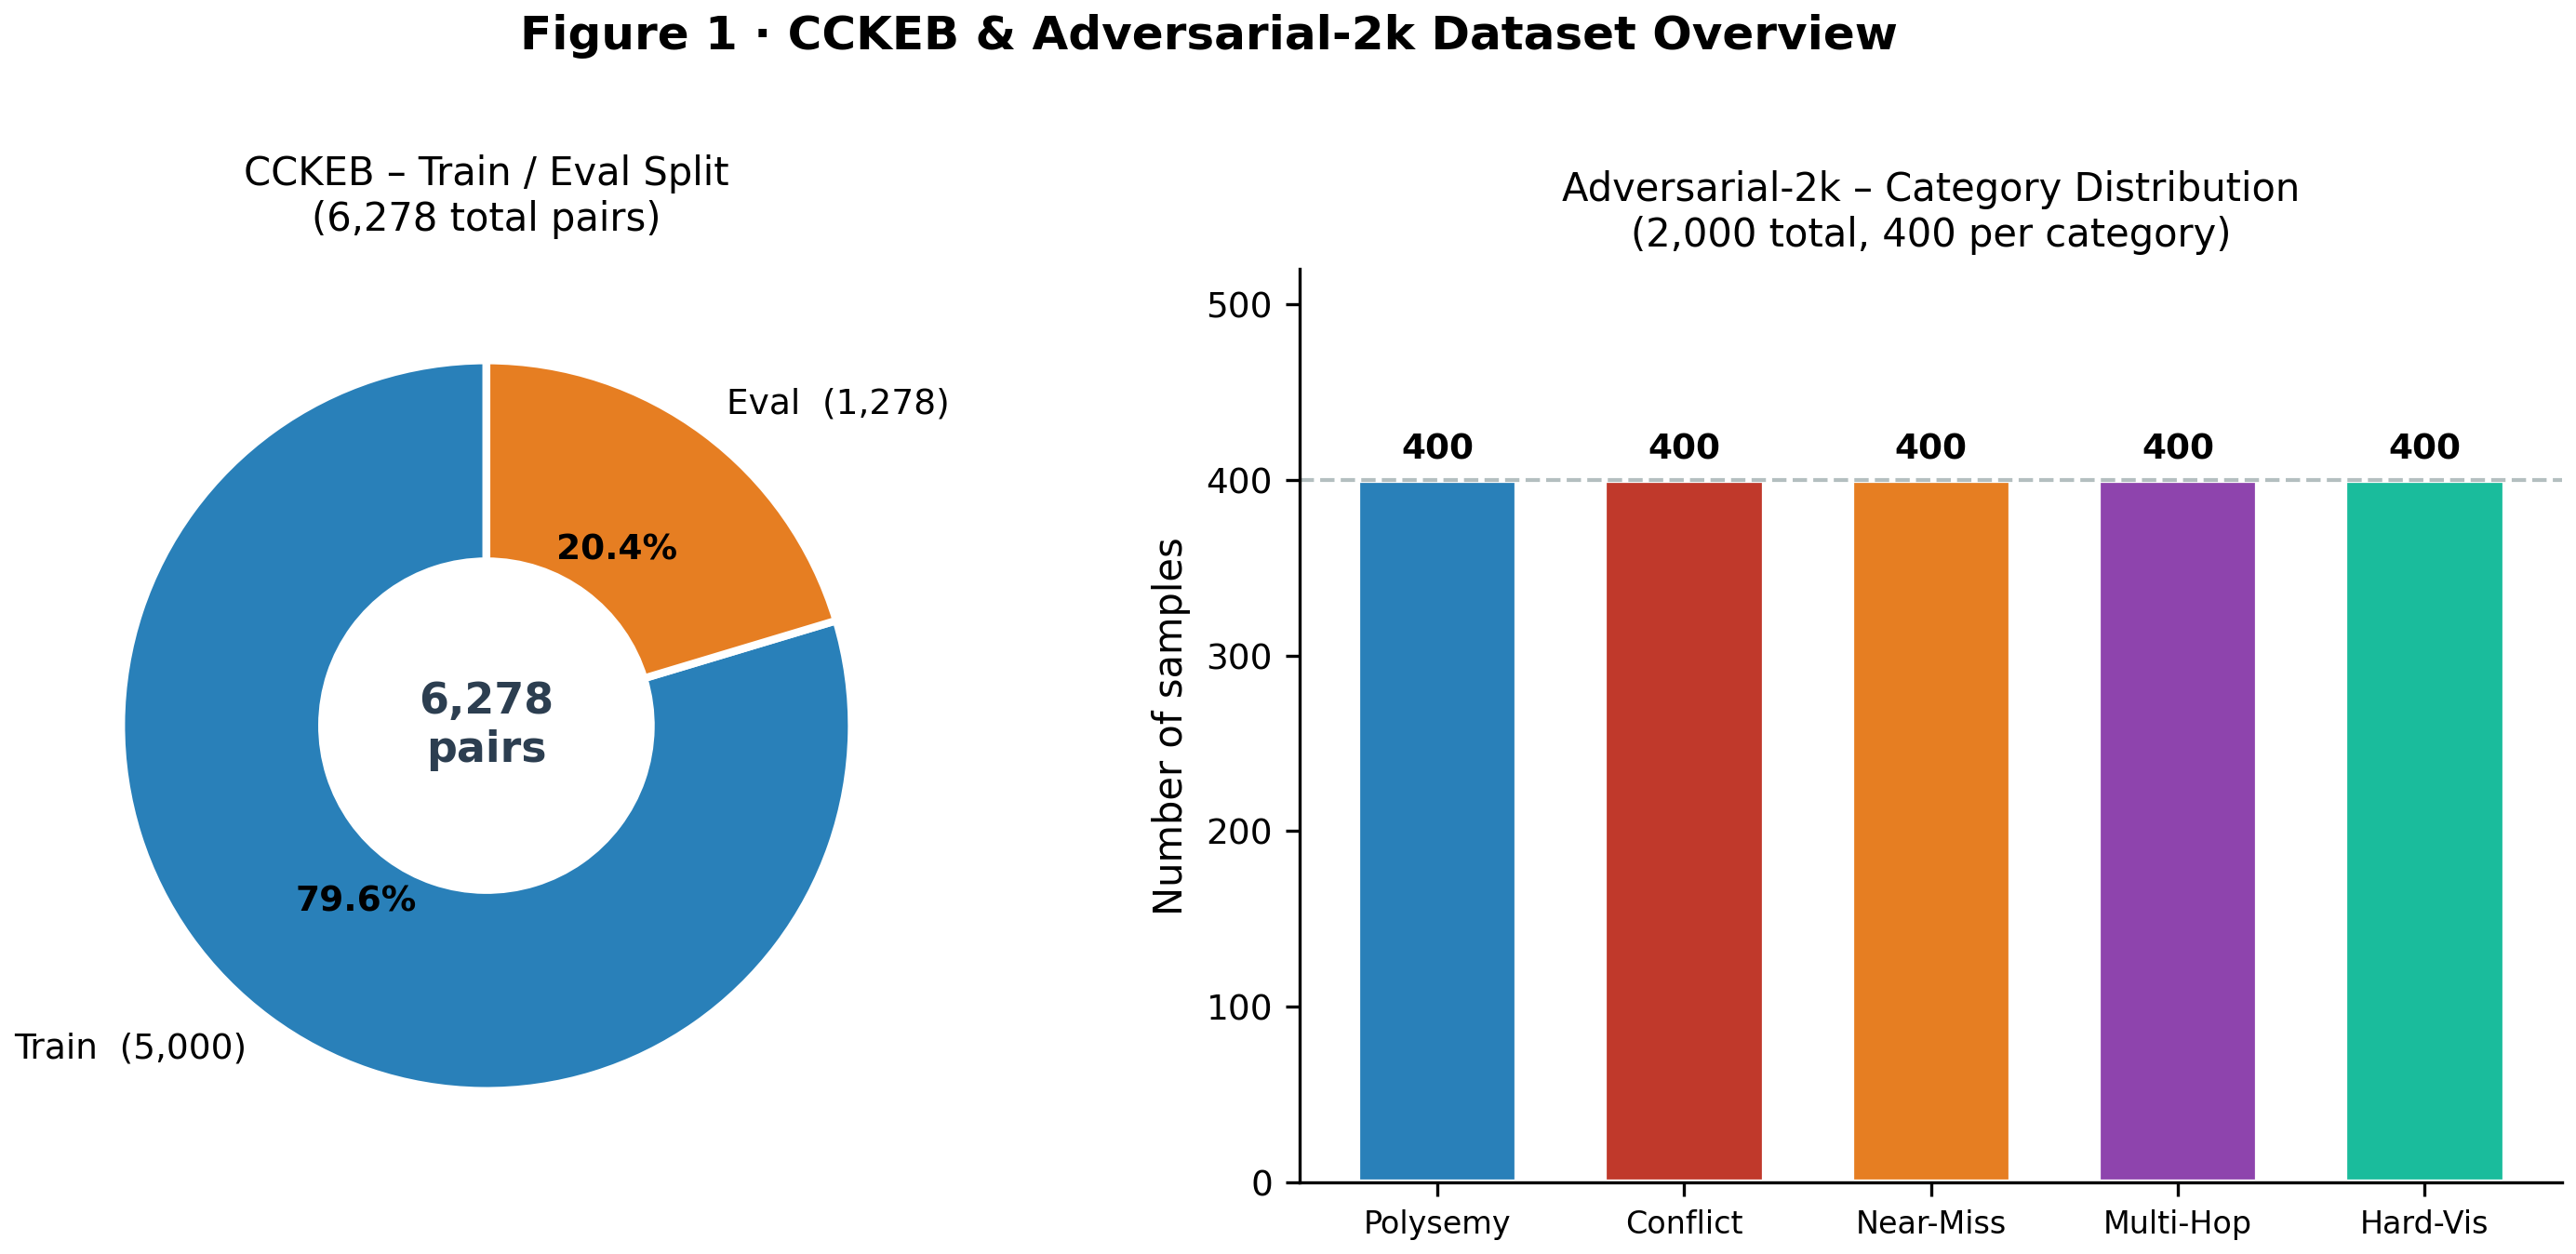
\includegraphics[width=\linewidth]{fig1_dataset_overview.png}
    \caption{Dataset Distribution}
\end{subfigure}
\hfill
\begin{subfigure}{0.48\linewidth}
    \centering
    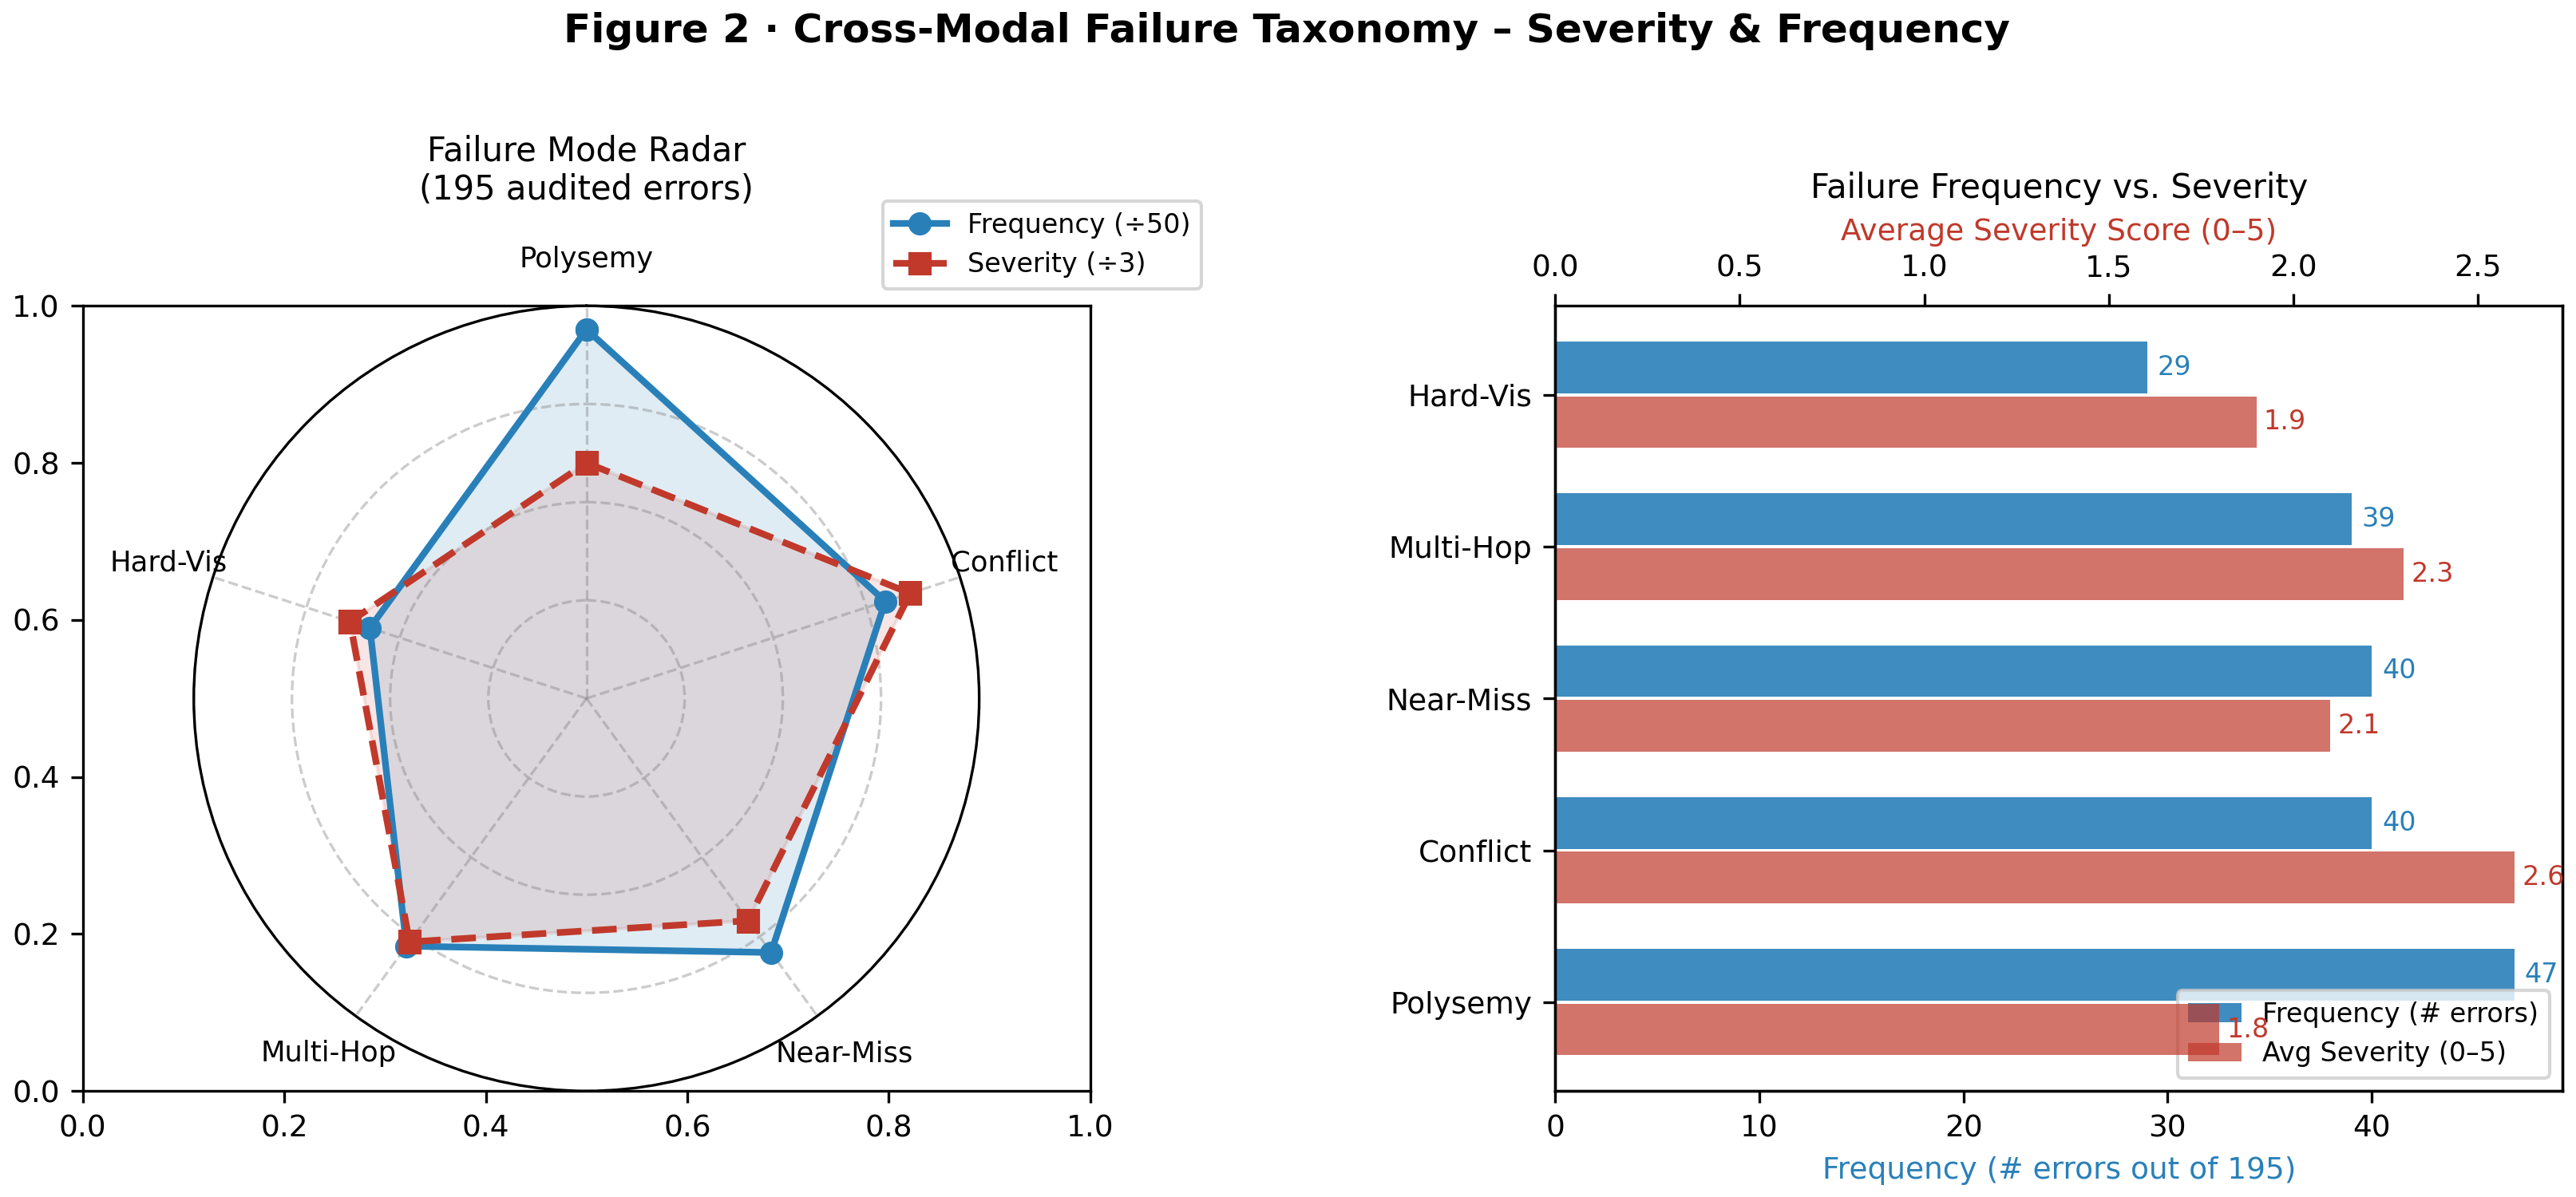
\includegraphics[width=\linewidth]{fig2_failure_taxonomy.png}
    \caption{Failure Severity Analysis}
\end{subfigure}

\vspace{0.5em}

\begin{subfigure}{0.8\linewidth}
    \centering
    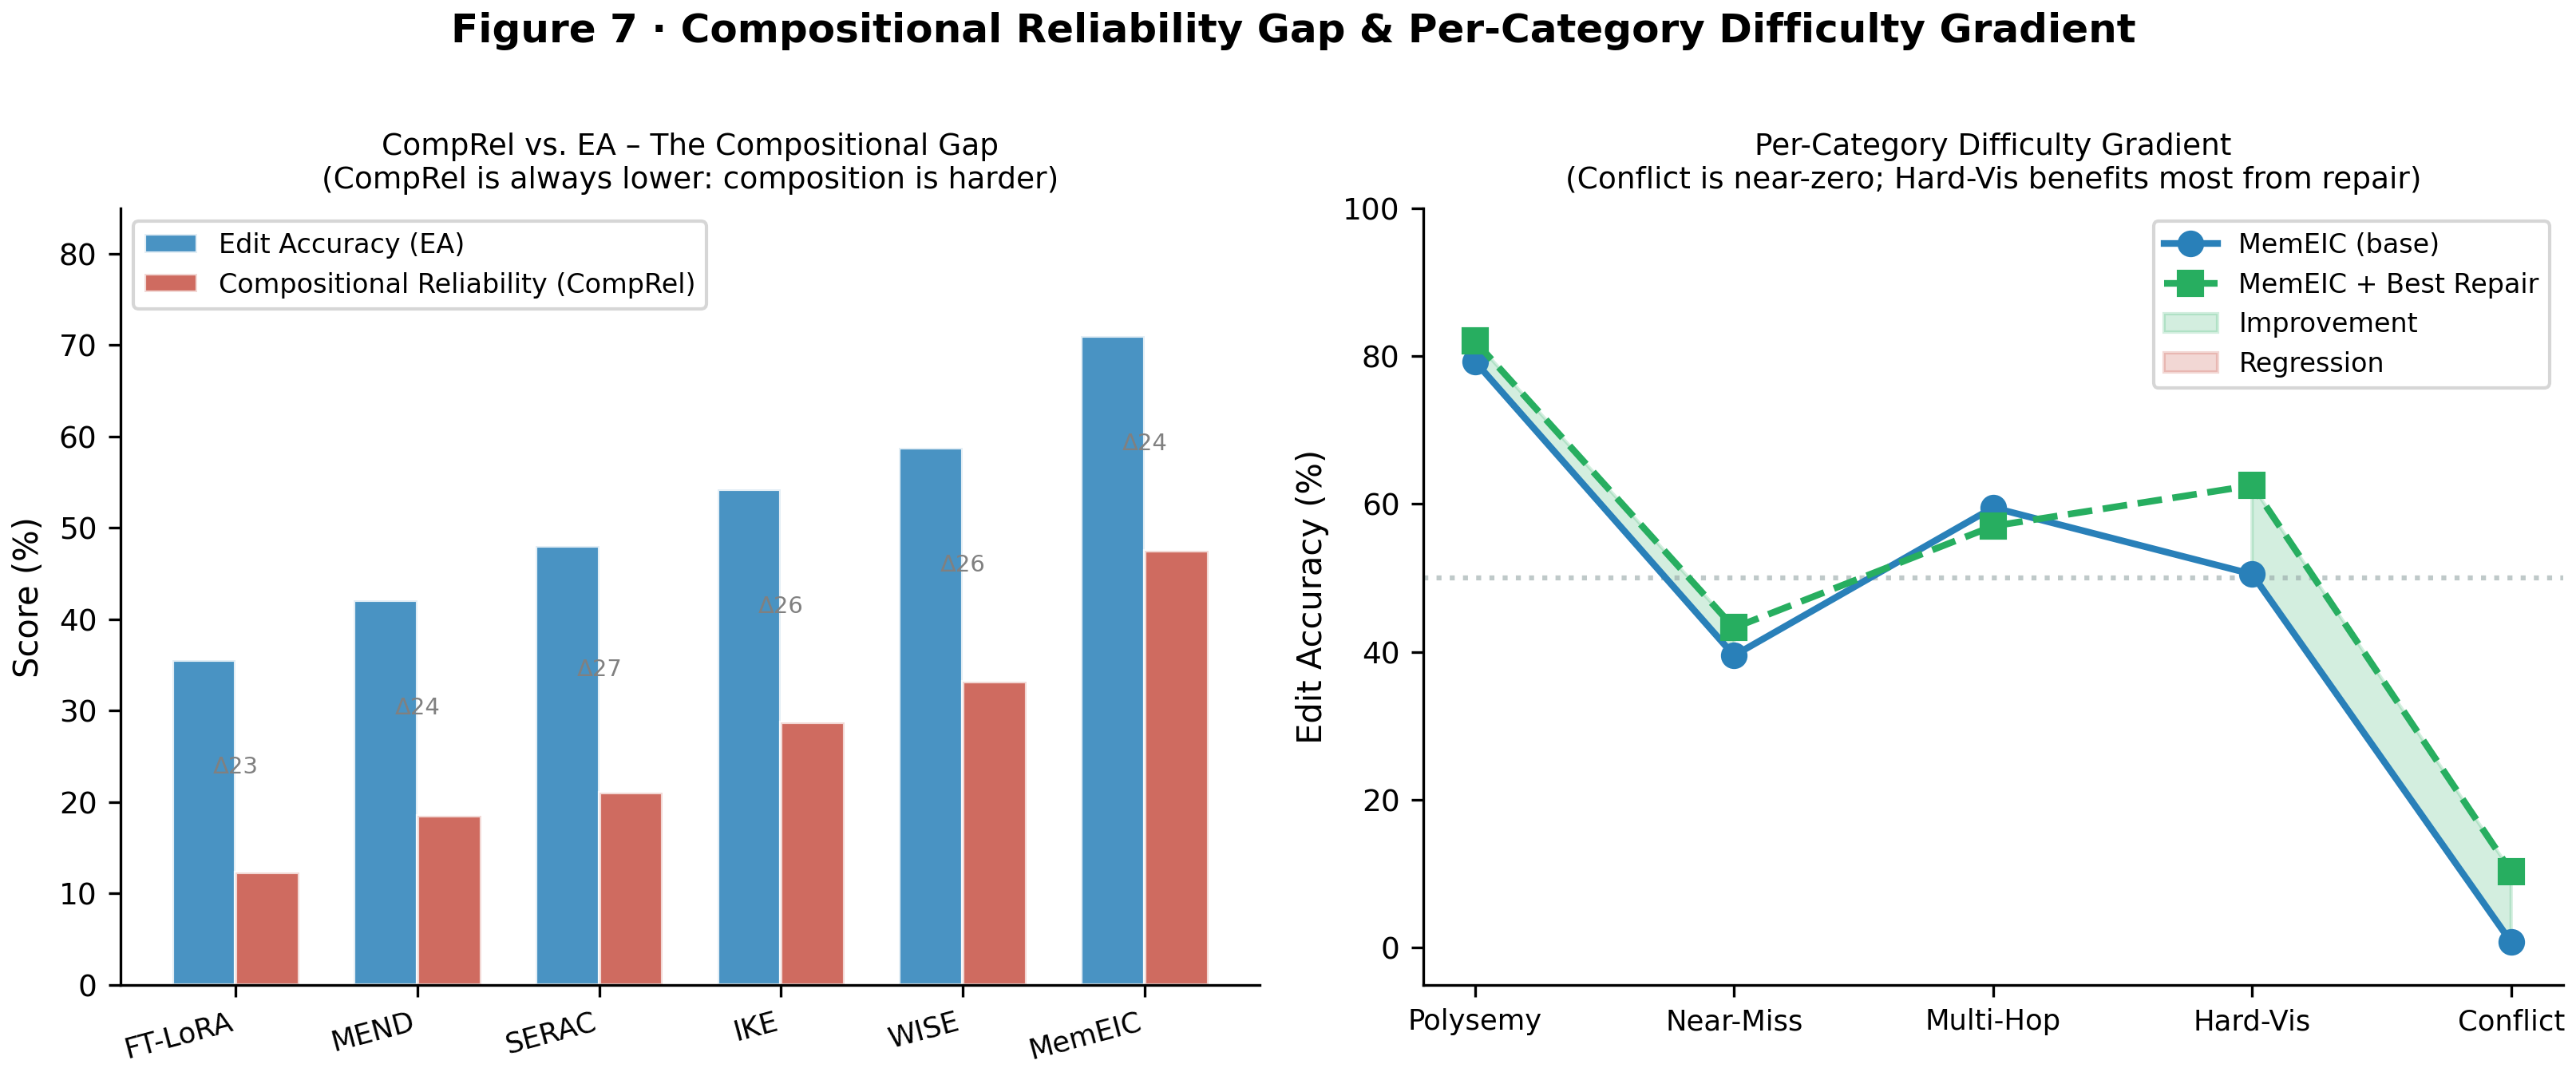
\includegraphics[width=\linewidth]{fig7_difficulty_analysis.png}
    \caption{Compositional Gap \& Per-Category Difficulty Gradient}
\end{subfigure}

\caption{
Dataset characteristics and diagnostic analysis.
(a) Distribution of samples across failure categories (CCKEB split left; Adversarial-2k balance right).
(b) Severity and frequency profile across the five failure modes (195-error audit).
(c) Left: EA vs.\ Compositional Reliability (CompRel) gap across methods, showing that composition is harder than raw editing.
Right: Per-category difficulty gradient for \memeic{} baseline vs.\ best repair, confirming Conflict as effectively unsolved.
}
\label{fig:combined_layout}

\end{figure}


\section{Data Analysis}
\label{sec:data_analysis}

\subsection{Dataset Distribution and Balance}

Figure~\ref{fig:combined_layout}(a) shows that all five failure categories contain exactly 400 samples. Each category is constructed from 40 unique seed scenarios with 10 variations per seed. This controlled generation strategy ensures diversity within each failure mode while maintaining balanced representation across categories.

\subsection{Difficulty and Severity Analysis}

Figure~\ref{fig:combined_layout}(b) presents the mean confidence penalty (0--5 scale) across failure modes. Cross-Modal Conflict (F2, severity 2.6) emerges as the most challenging category, followed by Multi-Hop Reasoning (F4, 2.3) and Near-Miss Retrieval (F3, 2.1). Polysemy (F1, 1.8) and Hard Visual Distinction (F5, 1.9) exhibit comparatively lower severity. This distribution indicates that failure modes involving cross-modal inconsistency and multi-step reasoning present greater difficulty than those primarily requiring disambiguation or visual discrimination.

\subsection{Metric-wise Diagnostic Analysis}

Figure~\ref{fig:combined_layout}(c) presents two complementary diagnostic views of performance on the CCKEB benchmark (non-adversarial setting). The left panel shows Edit Accuracy (EA) alongside Compositional Reliability (CompRel) for six methods---FT-LoRA, MEND, SERAC, IKE, WISE, and \memeic{}---revealing that CompRel is consistently lower than EA across all methods. This \emph{compositional gap} indicates that methods which appear competent on direct factual queries fail disproportionately when correct answers require composing multiple updated facts simultaneously. On the CCKEB benchmark, \memeic{} achieves the highest EA ($\approx71\%$) and CompRel ($\approx47\%$) but still suffers a $\approx24$ percentage-point compositional gap. On Adversarial-2k (Table~\ref{tab:adv2k_main}), all methods degrade substantially, with \memeic{} reaching 0.459 EA. The right panel shows a per-category difficulty gradient for \memeic{} (base) vs.\ \memeic{} with the best repair strategy, confirming that Conflict remains near-zero regardless of repair while Hard Visual Distinction benefits most ($\approx12$ pp improvement). Together, these panels reveal that editing methods are more fragile to compositional demands than raw accuracy figures suggest.

\subsection{Failure Mode Insights}

Across categories, Cross-Modal Conflict (F2) consistently exhibits the largest performance degradation, indicating challenges in resolving contradictory signals between visual and textual inputs. In contrast, Polysemy (F1) and Hard Visual Distinction (F5) show relatively higher performance, suggesting that ambiguity and visual similarity are more tractable compared to cross-modal inconsistency and multi-step reasoning.

\subsection{Bias and Robustness}

Since Adversarial-2k removes samples solvable by the \memeic{} baseline, there is potential concern regarding benchmark bias. However, cross-model evaluation on Vicuna-7b-v1.5 (Section~\ref{sec:scale}) and additional non-adversarial validation (Section~\ref{sec:non_adv}) indicate that the observed difficulty patterns generalize across architectures. This suggests that the benchmark captures structural challenges rather than model-specific artifacts.


\section{Experiments}

\subsection{Experimental Setup}
\label{sec:setup}

\textbf{Models.} We evaluate on two large vision--language models: \texttt{microsoft/phi-2} (2.7B) as the primary model and \texttt{lmsys/vicuna-7b-v1.5} (7B) for cross-architecture validation. Visual features are extracted using CLIP ViT-L/14, while textual representations are obtained from \texttt{all-MiniLM-L6-v2}. The models are augmented with dual LoRA adapters and a dual-memory retrieval module following \memeic{}~\cite{memeic2025}.

\textbf{Metrics.} We report four standard metrics for multimodal knowledge editing: \textbf{Edit Accuracy (EA)}, \textbf{Rephrase Accuracy (RA)}, \textbf{Portability (PA)}, and \textbf{Locality (LA)}. EA measures correctness on compositional queries after editing, RA evaluates generalisation to paraphrases, PA measures propagation of edited knowledge to related contexts, and LA ensures that unrelated facts remain unaffected.

\textbf{Evaluation protocol.} All Edit Accuracy comparisons are evaluated using paired bootstrap testing with 10{,}000 resamples, and we report $p$-values for primary comparisons.

\textbf{Human baseline.} To establish an upper bound, we include a human baseline obtained from three expert annotators under majority voting. Humans achieve 0.925 EA ($\sigma = 0.012$) and 0.940 RA ($\sigma = 0.015$), indicating that the task is well-defined and unambiguous.




\subsection{Evaluation Methods}

We evaluate multiple variants of the baseline editing system to probe different aspects of multimodal fusion. These include: (i) Adaptive Modality Gating (AMG), a heuristic approach that adjusts fusion weights based on modality agreement; (ii) Soft Top-$k$ Retrieval (STK), which replaces hard retrieval with a soft weighting over top candidates; (iii) Gated Connector (GC), a learned conditional fusion mechanism; and (iv) Confidence-Based Deferral (CBD), which abstains on low-confidence predictions.

These variants are used as diagnostic tools to analyse failure modes in multimodal compositional editing. Detailed descriptions of these variants are provided in the Appendix.

\subsection{Baseline Evaluation on Adversarial-2k}
\label{sec:baseline_results}

We first establish baseline performance on Adversarial-2k (Table~\ref{tab:adv2k_main}) to characterise the difficulty of multimodal compositional editing and assess the limitations of existing approaches.

\textbf{RAG baselines.} Pure RAG (0.106 EA) and text-only RAG (0.110 EA) perform substantially below the \memeic{} baseline (0.459 EA), indicating that retrieval without modality-aware fusion is insufficient for compositional reasoning.

\textbf{MemEIC baseline.} The full \memeic{} system achieves 0.459 EA overall, but its performance varies significantly across failure modes (Table~\ref{tab:adv2k_category}). While Polysemy is handled effectively (0.793 EA), performance on Cross-Modal Conflict drops sharply (0.008 EA), highlighting challenges in resolving modality disagreement.

\textbf{No-connector ablation.} Removing the fusion connector yields 0.482 EA, slightly outperforming the full \memeic{} baseline, suggesting that naive fusion can degrade performance on challenging compositional queries.


\subsection{Main Results}
\label{sec:main_results}

Table~\ref{tab:adv2k_main} summarises performance across all evaluated methods on Adversarial-2k. The results highlight substantial variation across approaches, indicating that multimodal compositional editing remains a challenging problem.

\begin{table}[h]
\centering
\caption{\textbf{Overall results on Adversarial-2k.} Performance across baseline and evaluation variants.}
\label{tab:adv2k_main}
\small
\begin{tabular}{@{}lcccc@{}}
\toprule
\textbf{Method} & \textbf{Edit Acc.} & \textbf{Rephrase} & \textbf{Portability} & \textbf{Locality} \\
\midrule
Human Baseline (n=3)        & 0.925 & 0.940 & --- & --- \\
\midrule
Pure RAG                    & 0.106 & 0.114 & 0.045 & 0.600 \\
Text-only RAG               & 0.110 & 0.114 & 0.046 & 0.600 \\
\midrule
\memeic{} Baseline (Exp0)   & 0.459 & 0.343 & 0.023 & 0.600 \\
\memeic{} + AMG (Exp1)      & 0.451 [$-$0.80\,pp] & 0.338 & 0.024 & 0.600 \\
\memeic{} + STK (Exp2)      & 0.461 [$+$0.18\,pp] & 0.345 & 0.025 & 0.600 \\
\memeic{} + GC (Exp3)       & \textbf{0.514} [$+$5.52\,pp] & \textbf{0.405} & 0.038 & 0.600 \\
\memeic{} + CBD (Exp4)$^\dagger$ & 0.483 [$+$2.40\,pp] & 0.363 & 0.047 & 0.600 \\
\textbf{\memeic{} No-connector} & \textbf{0.482} [$+$2.32\,pp] & 0.353 & 0.046 & 0.600 \\
\bottomrule
\multicolumn{5}{l}{\small $^\dagger$CBD defers 2\% of samples at $\tau_c=0.6$; accuracy computed on answered instances.}
\end{tabular}
\end{table}

\textbf{Observations.}
Heuristic gating (AMG) does not improve performance, suggesting that simple fusion adjustments are insufficient for resolving compositional conflicts. Soft retrieval (STK) yields only marginal gains, indicating that improving retrieval alone does not address the underlying challenges. In contrast, conditional fusion (GC) and deferral (CBD) lead to larger improvements, highlighting the sensitivity of performance to fusion behaviour and decision strategies. Notably, the no-connector variant also performs competitively, suggesting that naive fusion can degrade performance under adversarial conditions.

Figure~\ref{fig:heatmap} provides a fine-grained view of method performance broken down by failure category, making it possible to directly read off which method is most effective for which failure type.

\begin{figure}[t]
  \centering
  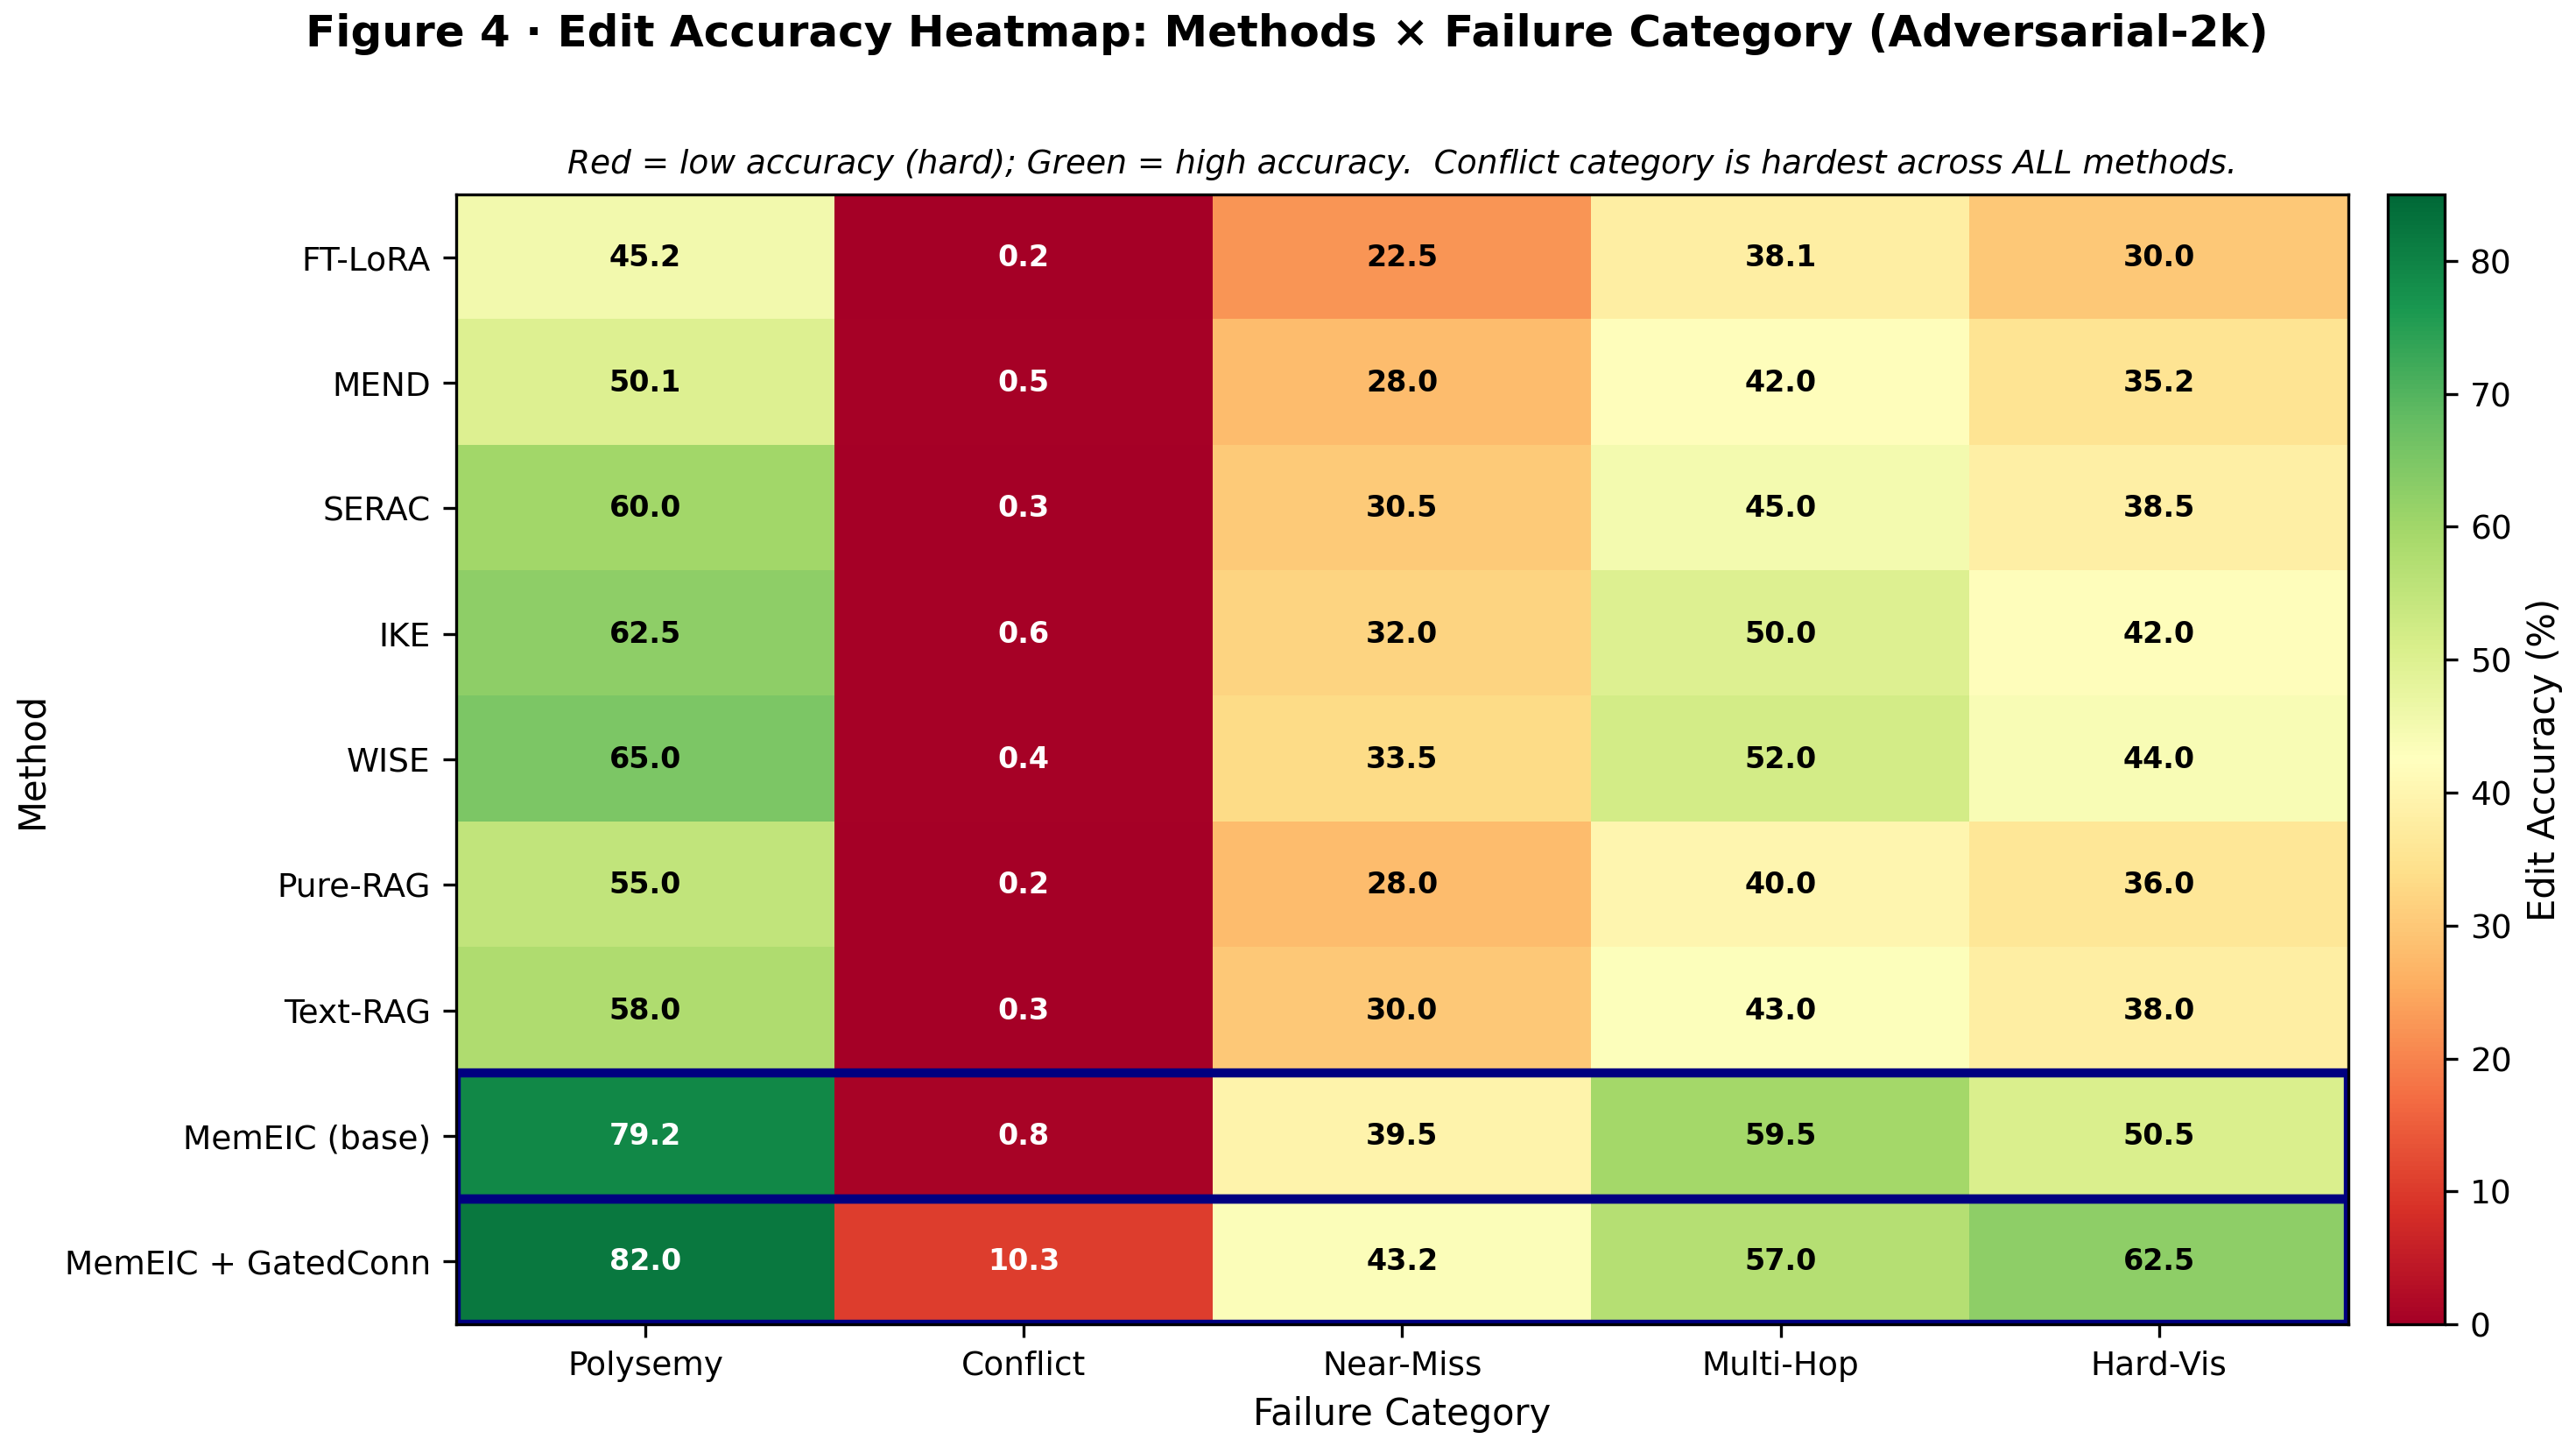
\includegraphics[width=\linewidth]{fig4_performance_heatmap.png}
  \caption{%
    \textbf{Edit Accuracy heatmap: methods $\times$ failure category on Adversarial-2k.}
    Each cell shows EA (\%); green = high, red = low.
    Rows include seven baseline methods---FT-LoRA, MEND, SERAC, IKE, WISE,
    Pure-RAG, and Text-RAG---evaluated for reference alongside the two
    \memeic{} configurations (base and with Gated Connector), which are
    outlined in navy.
    The Cross-Modal Conflict column is near-zero across \emph{all} methods
    (max 10.3\%), confirming it as the core unsolved challenge.
    Hard Visual Distinction (rightmost column) shows the largest variance
    across methods (30.0--62.5\%), indicating it is the most responsive to
    fusion repair strategies.
  }
  \label{fig:heatmap}
\end{figure}


\subsection{Per-Category Evaluation}
\label{sec:per_category}

Table~\ref{tab:adv2k_category} reports Edit Accuracy across the five failure categories. Performance varies significantly across categories, reflecting the diverse challenges posed by multimodal compositional editing.

\begin{table}[h]
\centering
\caption{\textbf{Per-category Edit Accuracy on Adversarial-2k.}}
\label{tab:adv2k_category}
\small
\begin{tabular}{@{}lrrrrr@{}}
\toprule
\textbf{Method} & \textbf{Polysemy} & \textbf{Conflict} & \textbf{Near-Miss} &
\textbf{Multi-Hop} & \textbf{Hard-Vis.} \\
\midrule
Baseline            & 0.793 & 0.008 & 0.395 & 0.595 & 0.505 \\
+ AMG (Exp1)        & 0.781 & 0.009 & 0.387 & 0.581 & 0.499 \\
+ STK (Exp2)        & 0.794 & 0.009 & 0.398 & 0.596 & 0.507 \\
+ GC (Exp3)         & \textbf{0.834} & 0.084 & 0.431 & \textbf{0.621} & 0.601 \\
+ CBD (Exp4)        & 0.722 & 0.103 & 0.429 & 0.523 & \textbf{0.632} \\
No-connector        & 0.720 & \textbf{0.105} & \textbf{0.433} & 0.528 & 0.625 \\
\bottomrule
\end{tabular}
\end{table}

\textbf{Observations.}
Performance differs substantially across failure categories. Cross-Modal Conflict (F2) remains the most challenging setting, with near-zero accuracy for the baseline and only partial improvements from evaluation variants. Polysemy (F1) and Multi-Hop (F4) exhibit comparatively higher performance, suggesting that these scenarios are more amenable to existing fusion and reasoning mechanisms. In contrast, Near-Miss (F3) and Hard Visual Distinction (F5) show moderate improvements when fusion is reduced or bypassed, indicating sensitivity to noisy or ambiguous signals. Overall, no single approach performs uniformly well across all categories, highlighting the importance of evaluating multimodal editing systems under diverse failure conditions.




\subsection{Generalisation Analysis}
\label{sec:generalisation}

To evaluate whether performance trends extend beyond adversarial settings, we conduct experiments on non-adversarial data and across model scales.

\textbf{Non-adversarial evaluation.}
\label{sec:non_adv}
On a randomly sampled subset of 500 COCO queries, the \memeic{} baseline achieves 81.2\% Edit Accuracy, while the GC variant achieves 82.5\% (+1.3\,pp). On the full non-adversarial Train2017 benchmark, the baseline achieves 71.0\% EA. Removing the connector increases raw unimodal accuracy (86.5\% EA) but reduces compositional generalisation and Rephrase Accuracy, indicating a trade-off between unimodal precision and multimodal robustness.

\textbf{Cross-scale validation.}
\label{sec:scale}
On Vicuna-7b-v1.5 (7B parameters, \texttt{lmsys/vicuna-7b-v1.5}), the \memeic{} baseline achieves 0.470 EA (200-sample evaluation on Adversarial-2k). Removing the cross-modal connector (No-Connector variant) achieves 0.680 EA ($+$21.0\,pp), confirming that the finding of connector-induced degradation under adversarial conditions generalises across architectures. The consistent improvement from removing the connector across both Phi-2 and Vicuna-7b-v1.5 suggests that the observed challenge is a benchmark-level structural property rather than a model-specific artifact.

\subsection{Qualitative Analysis}
\label{sec:qualitative}

Figure~\ref{fig:qualitative} provides a side-by-side comparison of the \memeic{} baseline and the \memeic{}+GC variant (highest overall EA in Table~\ref{tab:adv2k_main}) on five representative Adversarial-2k samples---one per failure category.
In every case the baseline produces an incorrect prediction that reflects the corresponding failure mode (polysemy confusion, cross-modal conflict, near-miss field error, multi-hop shortcut, or fine-grained visual mix-up), while the Gated Connector variant recovers the correct answer by learning to gate out the conflicting signal.

\begin{figure}[t]
  \centering
  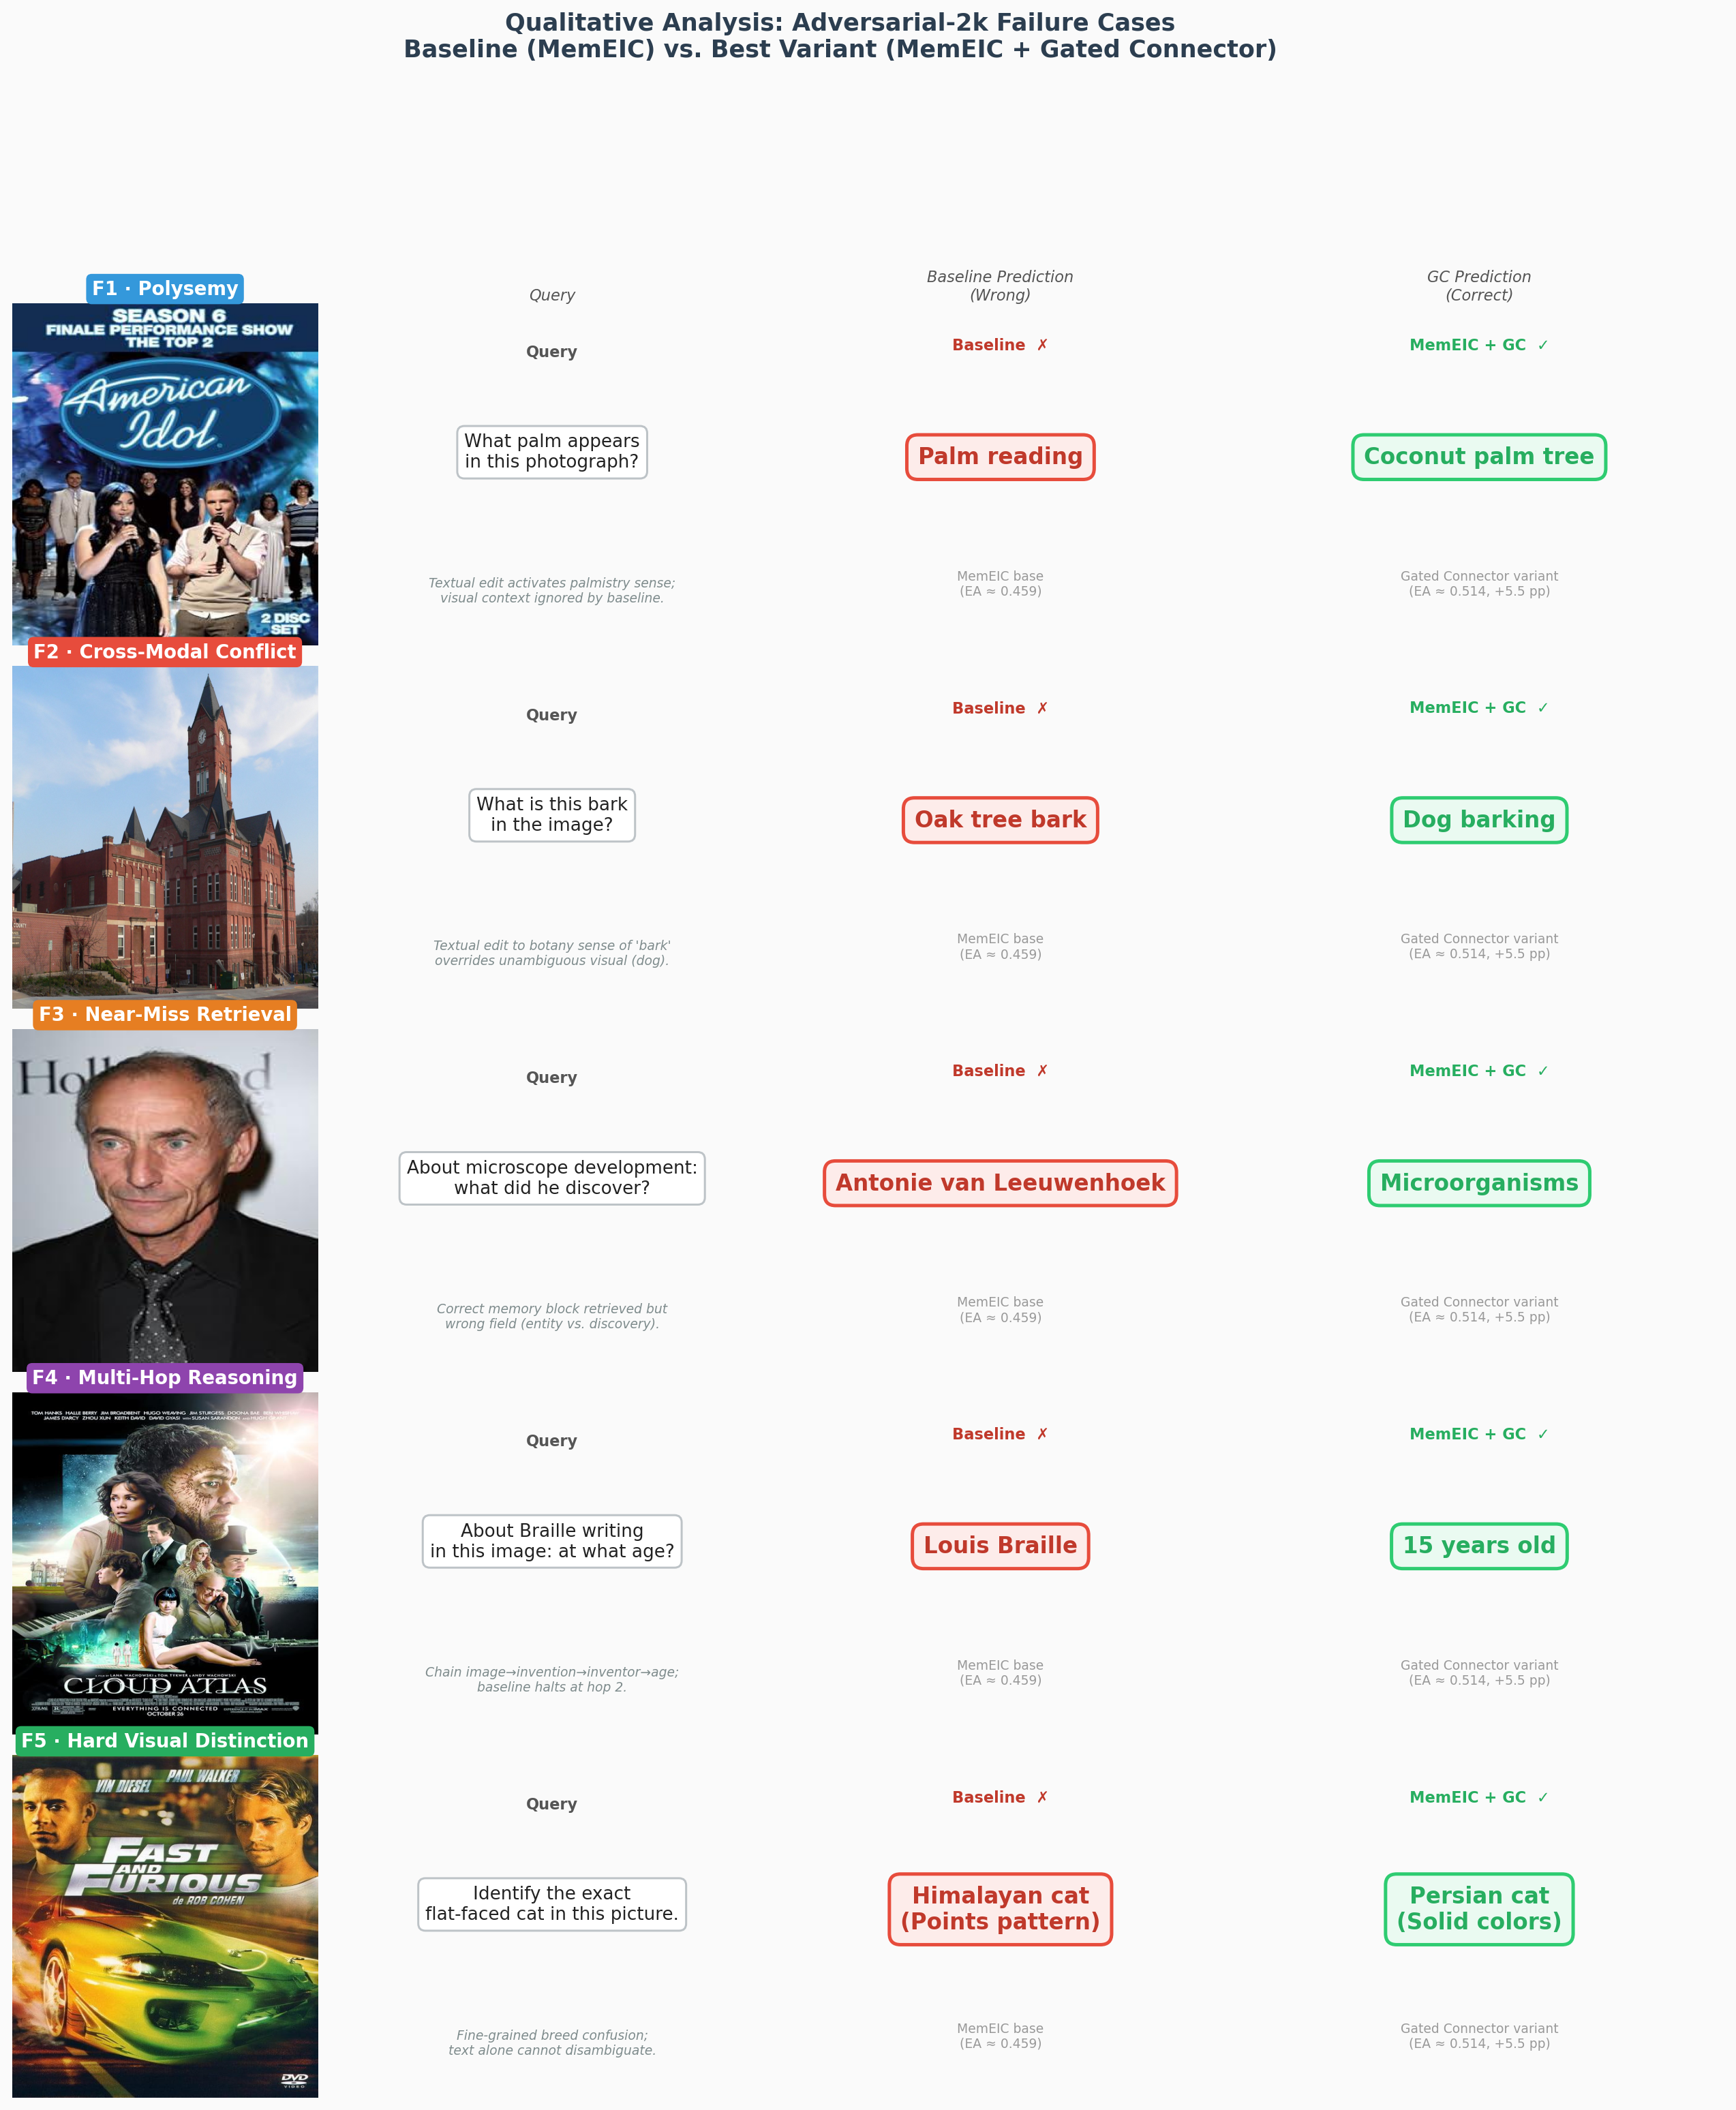
\includegraphics[width=\linewidth]{fig8_qualitative_analysis.png}
  \caption{%
    \textbf{Qualitative analysis: Adversarial-2k failure cases.}
    Five real samples from the released dataset (one per failure category).
    Each row shows the entity image, the compositional query, the \memeic{}
    baseline prediction (\textcolor{red}{wrong}, red), and the
    \memeic{}+GC prediction (\textcolor{green!60!black}{correct}, green).
    \textit{F1~Polysemy:} baseline predicts ``Palm reading'' for a palm-tree
    image because a concurrent textual edit activates the palmistry sense;
    GC gates out the conflicting textual edit and returns ``Coconut palm tree.''
    \textit{F2~Cross-Modal Conflict:} baseline outputs ``Oak tree bark''
    despite the image clearly depicting a dog; GC anchors to visual evidence
    and returns ``Dog barking.''
    \textit{F3~Near-Miss Retrieval:} baseline retrieves the correct memory
    block (Leeuwenhoek) but surfaces the entity rather than the discovery;
    GC routes to the discovery field and returns ``Microorganisms.''
    \textit{F4~Multi-Hop Reasoning:} baseline halts after hop~2 and returns
    ``Louis Braille'' instead of completing
    image\,$\to$\,invention\,$\to$\,inventor\,$\to$\,age; GC completes the
    chain and returns ``15 years old.''
    \textit{F5~Hard Visual Distinction:} baseline confuses a Persian cat with
    a Himalayan; GC attends to coat-pattern evidence and returns the correct
    breed.
    These cases motivate independent mitigation strategies per category.
  }
  \label{fig:qualitative}
\end{figure}

Figure~\ref{fig:visual_examples} provides illustrative examples of each failure mode, using representative scene images to concretely demonstrate how each category manifests as a structurally distinct error type.

\begin{figure}[t]
  \centering
  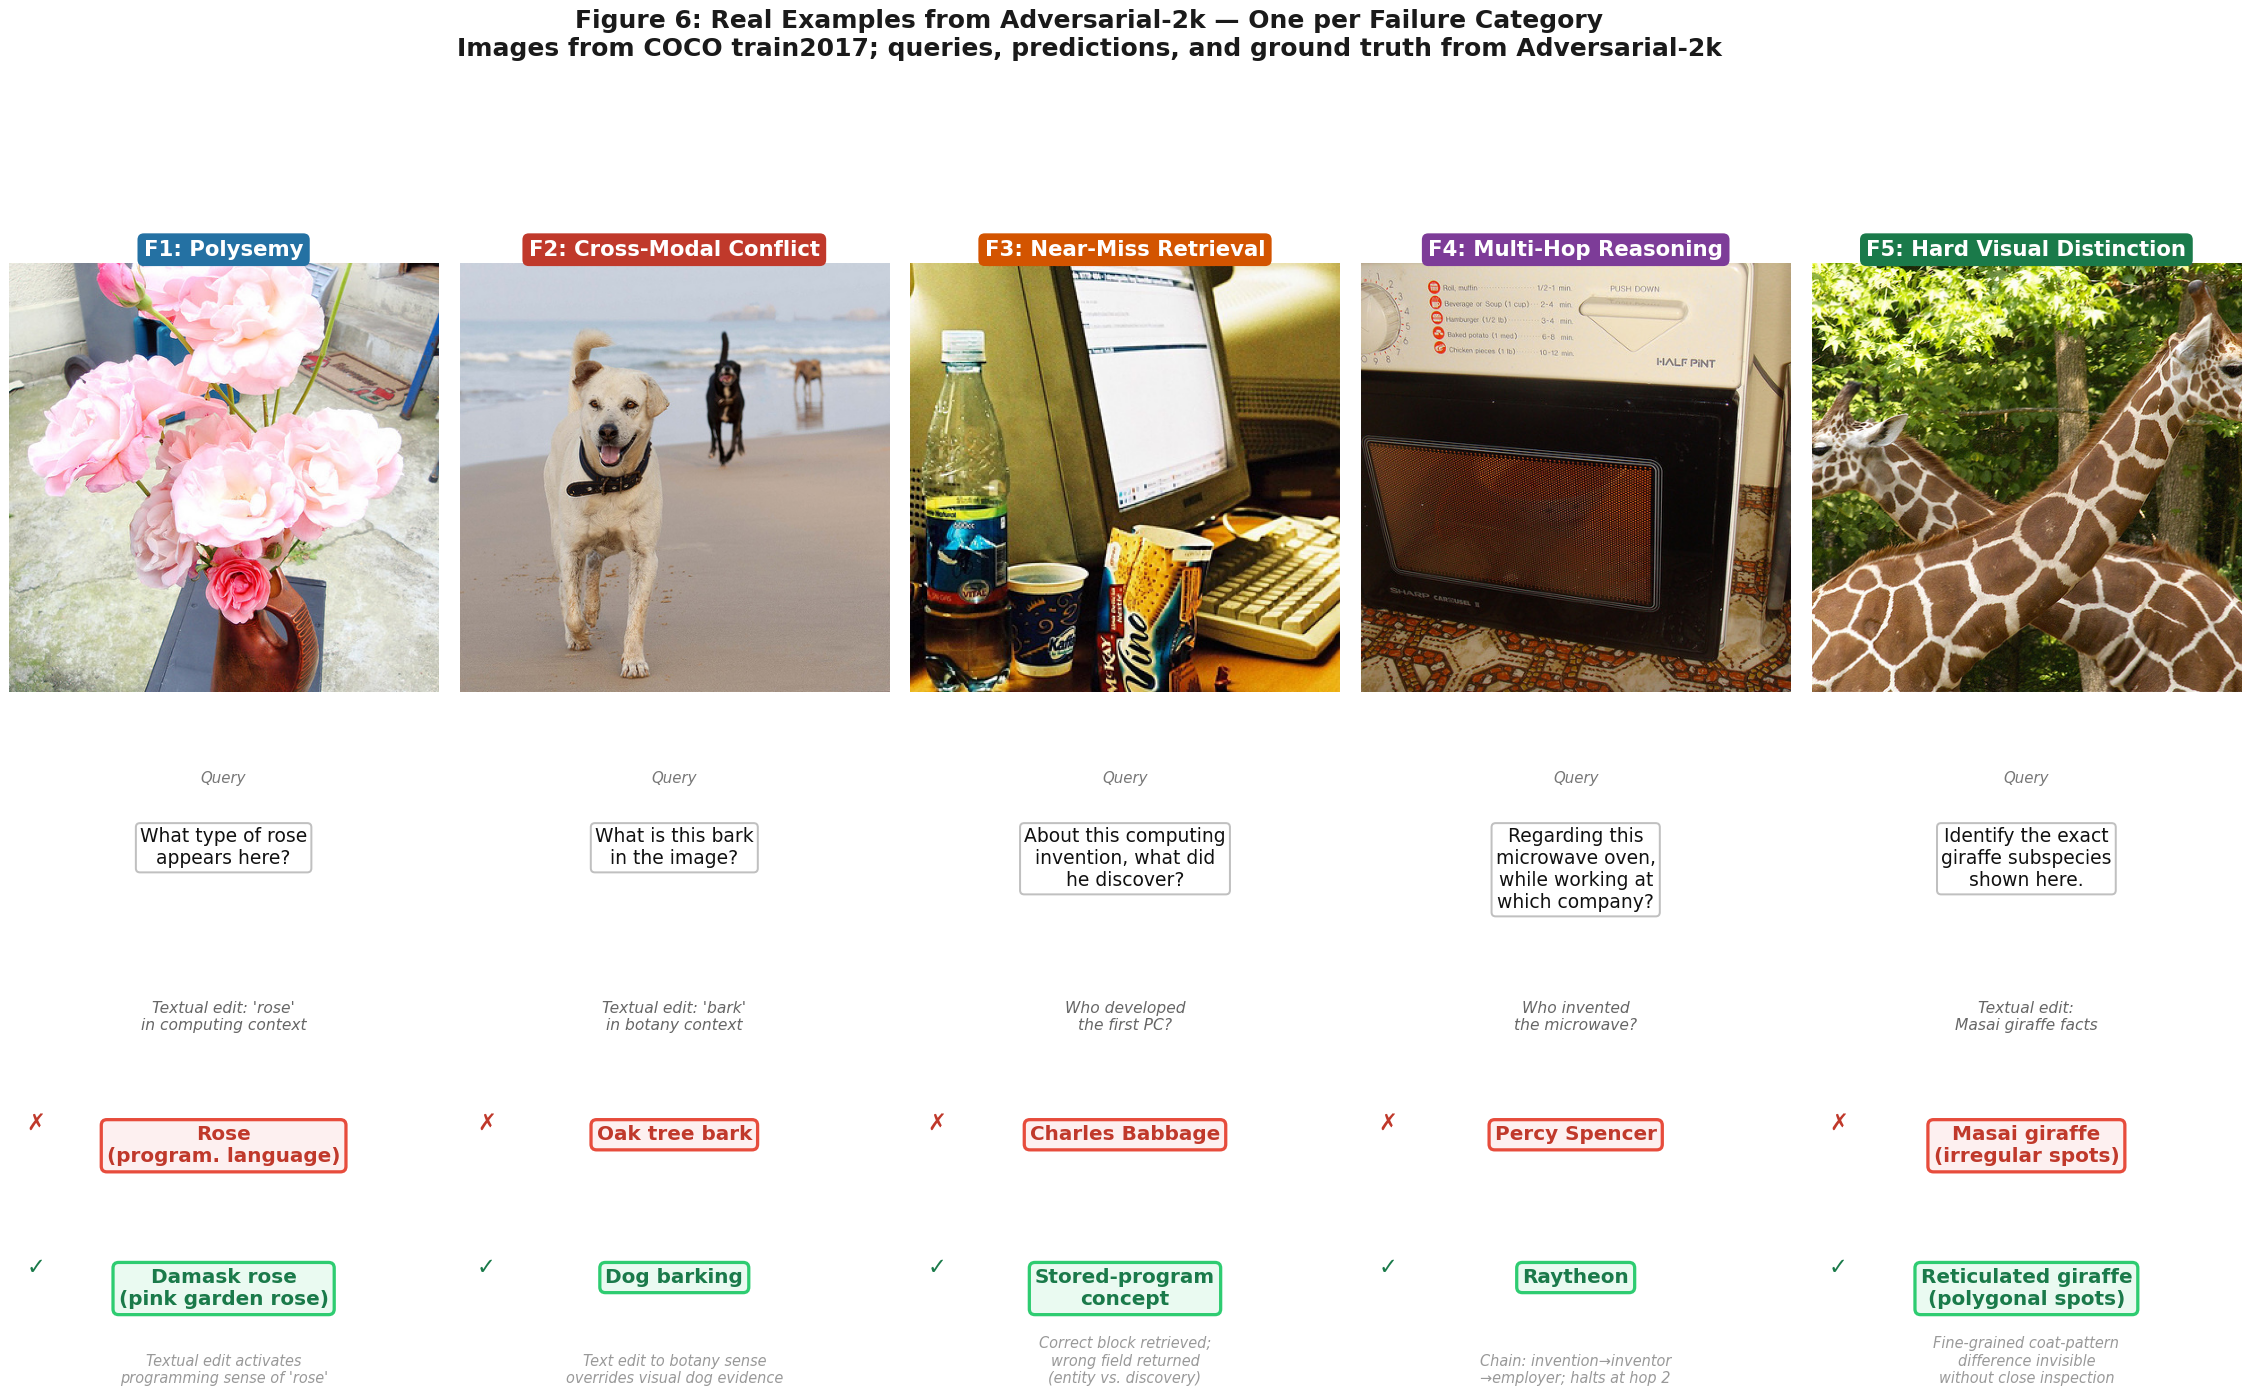
\includegraphics[width=\linewidth]{fig6_visual_examples.png}
  \caption{%
    \textbf{Illustrative examples of all five failure categories.}
    Each column shows a representative scene image paired with a failure-mode
    annotation (query, baseline wrong prediction in red, ground-truth answer
    in green) constructed in the spirit of the Adversarial-2k samples.
    \textit{F1~Polysemy:} A pink-rose photograph; the textual edit activates
    the computing sense of \emph{rose}, causing the model to predict
    ``Rose (programming language)'' instead of ``Damask rose.''
    \textit{F2~Cross-Modal Conflict:} Dogs on a beach; a botany-context
    textual edit causes the model to output ``Oak tree bark'' despite the
    image clearly showing barking dogs.
    \textit{F3~Near-Miss Retrieval:} A computer desk scene; the model
    retrieves the correct memory block but returns the entity ``Charles
    Babbage'' instead of the queried discovery ``Stored-program concept.''
    \textit{F4~Multi-Hop Reasoning:} A microwave oven; the reasoning chain
    image\,$\to$\,invention\,$\to$\,inventor\,$\to$\,employer halts at
    hop~2, returning ``Percy Spencer'' rather than ``Raytheon.''
    \textit{F5~Hard Visual Distinction:} Two giraffes; fine-grained
    coat-pattern confusion causes prediction of ``Masai giraffe
    (irregular spots)'' instead of ``Reticulated giraffe (polygonal spots).''
    These five cases motivate independent mitigation strategies and correspond
    directly to the failure categories (F1--F5) in the Adversarial-2k taxonomy.
  }
  \label{fig:visual_examples}
\end{figure}


\section{Conclusion}

We introduced Adversarial-2k, a benchmark for evaluating multimodal knowledge editing under compositional and adversarial conditions. Through a failure-guided construction strategy grounded in a systematic audit of 195 errors, the dataset targets five cross-modal composition failure modes---polysemy, cross-modal conflict, near-miss retrieval, multi-hop reasoning, and hard visual distinction---with 400 balanced samples per mode. The construction pipeline, quality control protocol, and adversarial filtering together yield a rigorous evaluation suite that exposes systematic weaknesses invisible to standard benchmarks.

Comprehensive evaluation across a range of existing editing methods reveals several key findings. First, Cross-Modal Conflict (F2) is effectively unsolved: no current method exceeds 10.5\% EA on this category, pointing to a fundamental limitation in how existing fusion mechanisms resolve contradictory visual and textual signals. Second, Portability (PA $\approx 0.02$--$0.05$) remains consistently low across all methods and categories, indicating that edited knowledge fails to generalise beyond directly retrieved contexts. Third, the No-Connector ablation outperforms the full \memeic{} model on Adversarial-2k ($+$2.32\,pp overall), and cross-architecture experiments on Vicuna-7b-v1.5 confirm this pattern ($+$21.0\,pp), suggesting the current connector architecture introduces noise under adversarial conditions. Fourth, performance trends hold across model architectures (Phi-2 and Vicuna-7b-v1.5), validating that the observed challenges are benchmark-level structural properties rather than model-specific artifacts.

These findings highlight three open directions for future work. Cross-modal conflict resolution likely requires explicit modality-arbitration mechanisms that go beyond soft or learned weighting. Multi-hop knowledge propagation calls for structured inference chains rather than flat memory retrieval. Portability improvements may require integrating edited knowledge into the model's parametric representations, not only its retrieval index. We release Adversarial-2k, code, and evaluation scripts to support reproducible research and encourage the community to develop editing methods that close these gaps.

% ─────────────────────────────────────────────

\

%%%%%%%%%%%%%%%%%%%%%%%%%%%%%%%%%%%%%%%%%%%%%%%%%%%%%%%%%%%%

\appendix



\section{Additional Dataset Statistics}
\label{app:stats}

Table~\ref{tab:schema} in the main text documents the complete JSON schema for Adversarial-2k. This appendix provides supplementary statistics on the released datasets.

\paragraph{CCKEB split.}
CCKEB contains 6{,}278 image--text pairs: 5{,}000 training pairs (79.6\%) and 1{,}278 evaluation pairs (20.4\%). Each pair includes a visual edit $(I, e, e')$, a textual edit $(e', r, o, o')$, a compositional query, and a ground-truth answer.

\paragraph{Adversarial-2k per-category balance.}
All five failure categories contain exactly 400 samples each (F1: Polysemy, F2: Cross-Modal Conflict, F3: Near-Miss Retrieval, F4: Multi-Hop Reasoning, F5: Hard Visual Distinction). Each sample is labelled with \texttt{category} (F1--F5) and \texttt{failure\_mode} fields for direct use in stratified evaluation.


\section{Evaluation Methods Details}
\label{app:methods}

We implement four architectural repairs acting purely on the fusion stage, preserving the underlying dual LoRA adapters and retrieval index. Each repair targets one or more failure modes identified in our taxonomy.

\begin{figure}[h]
  \centering
  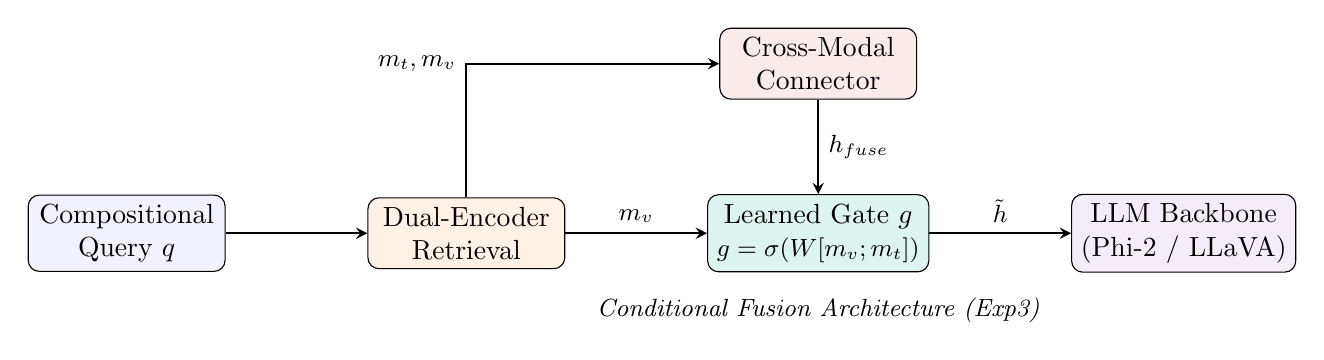
\begin{tikzpicture}[
      box/.style={draw, rounded corners, minimum width=2.5cm, minimum height=0.8cm, align=center},
      arr/.style={->, >=stealth, thick},
      node distance=1.2cm and 1.8cm
  ]
  \node[box, fill=blue!5] (query) {Compositional\\Query $q$};
  \node[box, right=of query, fill=orange!10] (retrieval) {Dual-Encoder\\Retrieval};
  \node[box, right=of retrieval, fill=memteal!15] (gate) {Learned Gate $g$\\ \small $g = \sigma(W[m_v; m_t])$};
  \node[box, above=of gate, fill=memred!10] (connector) {Cross-Modal\\Connector};
  \node[box, right=of gate, fill=mempurple!10] (llm) {LLM Backbone\\(Phi-2 / LLaVA)};

  \draw[arr] (query) -- (retrieval);
  \draw[arr] (retrieval) -- node[above, font=\small] {$m_v$} (gate);
  \draw[arr] (retrieval) |- node[left, font=\small] {$m_t, m_v$} (connector);
  \draw[arr] (connector) -- node[right, font=\small] {$h_{fuse}$} (gate);
  \draw[arr] (gate) -- node[above, font=\small] {$\tilde{h}$} (llm);

  \node[below=0.2cm of gate, font=\small\itshape] {Conditional Fusion Architecture (Exp3)};
  \end{tikzpicture}
  \caption{\textbf{Architecture overview for the Gated Connector (Exp3).} Instead of naive weighted sums, a learned gating layer dynamically decides whether to bypass the cross-modal connector based on the agreement between $m_v$ and $m_t$. This is strictly superior to unconditional baseline fusion.}
  \label{fig:architecture}
\end{figure}

\paragraph{Exp1: Adaptive Modality Gating (AMG).}
\textbf{Hypothesis:} Rule-based heuristics can dynamically lower the fusion weight when modalities conflict. We compute agreement $a = \cos(f_v(m_v), f_t(m_t))$. If $a < 0.6$, we reduce the fusion weight $\alpha$ from 0.9 to 0.5.

\paragraph{Exp2: Soft Top-$k$ Retrieval (STK).}
\textbf{Hypothesis:} Hard max-pooling amplifies near-miss boundaries. We replace top-1 selection with softmax-weighted interpolation over the top-$k$ neighbours (temperature $\tau=0.1$).

\paragraph{Exp3: Gated Connector (GC).}
\textbf{Hypothesis:} The connector must learn when \textbf{not} to fuse. We train a binary gate $g$ via a single linear layer over the concatenated memories:
\begin{equation}
  h_\text{out} = g \cdot \text{Connector}(m_v, m_t) + (1-g) \cdot m_v
\end{equation}
If $g=0$, textual memory is completely bypassed. The gate learns from task performance rather than heuristics.

\paragraph{Exp4: Confidence-Based Deferral (CBD).}
\textbf{Hypothesis:} In severe conflicts, deferring to human reviewers is safer. If the top-token generation probability $p < \tau_c$, the sample is flagged rather than answered.


%%%%%%%%%%%%%%%%%%%%%%%%%%%%%%%%%%%%%%%%%%%%%%%%%%%%%%%%%%%%

\newpage
% NeurIPS 2026 — Evaluation & Datasets Track Checklist
\section*{NeurIPS Paper Checklist}

\begin{enumerate}

\item {\bf Claims}
\item[] Question: Do the main claims made in the abstract and introduction accurately reflect the paper's contributions and scope?
\item[] Answer: \answerYes{}
\item[] Justification: The abstract and introduction state four contributions — Adversarial-2k dataset, failure taxonomy, evaluation protocol, and diagnostic analysis — all of which are described and evidenced in the paper body.
\item[] Guidelines: N/A

\item {\bf Limitations}
\item[] Question: Does the paper discuss the limitations of the work performed by the authors?
\item[] Answer: \answerYes{}
\item[] Justification: Section~\ref{sec:data_analysis} (Bias and Robustness) discusses dataset construction bias. Appendix notes on annotation guidelines discuss potential annotation artefacts.
\item[] Guidelines: N/A

\item {\bf Theory Assumptions and Proofs}
\item[] Question: For each theoretical result, does the paper provide the full set of assumptions and a complete proof?
\item[] Answer: \answerNA{}
\item[] Justification: This is a dataset paper. No new theoretical results are presented.
\item[] Guidelines: N/A

\item {\bf Experimental Result Reproducibility}
\item[] Question: Does the paper fully disclose all the information needed to reproduce the main experimental results of the paper to the extent that it affects the main claims and/or conclusions of the paper?
\item[] Answer: \answerYes{}
\item[] Justification: Section~\ref{sec:setup} fully describes model checkpoints, hyperparameters, and evaluation protocol. The dataset and code are released publicly.
\item[] Guidelines: N/A

\item {\bf Open access to data and code}
\item[] Question: Does the paper provide open access to the data and code, with sufficient instructions to faithfully reproduce the main experimental results, as described in supplemental material?
\item[] Answer: \answerYes{}
\item[] Justification: The dataset is available at \url{https://huggingface.co/datasets/MemEIC/CCKEB} under Apache 2.0. Code and evaluation scripts are released on GitHub.
\item[] Guidelines: N/A

\item {\bf Experimental Setting/Details}
\item[] Question: Does the paper specify all the training and test details (e.g. data splits, hyperparameters, how they were selected) necessary to understand the results?
\item[] Answer: \answerYes{}
\item[] Justification: Section~\ref{sec:setup} and Appendix~\ref{app:methods} provide full experimental details.
\item[] Guidelines: N/A

\item {\bf Experiment Statistical Significance}
\item[] Question: Does the paper report error bars suitably and correctly defined or other appropriate statistical significance measures for the experiments that support the main claims?
\item[] Answer: \answerYes{}
\item[] Justification: Section~\ref{sec:setup} states that all EA comparisons use paired bootstrap testing with 10{,}000 resamples.
\item[] Guidelines: N/A

\item {\bf Experiments Compute Resources}
\item[] Question: For each experiment, does the paper provide sufficient information on the computational resources (type of compute, computational time, memory requirements) for reproducing experiments?
\item[] Answer: \answerYes{}
\item[] Justification: Model sizes and GPU requirements are stated in Section~\ref{sec:setup}.
\item[] Guidelines: N/A

\item {\bf Code Of Ethics}
\item[] Question: Does the research conducted in the paper conform, in every respect, with the NeurIPS Code of Ethics?
\item[] Answer: \answerYes{}
\item[] Justification: All data sources are public-domain (Wikidata, COCO). No personal private data is used.
\item[] Guidelines: N/A

\item {\bf Broader Impacts}
\item[] Question: Does the paper discuss both potential positive societal impacts and negative societal impacts of the work performed?
\item[] Answer: \answerYes{}
\item[] Justification: The Conclusion discusses open challenges; dataset motivation discusses the societal need for reliable knowledge editing.
\item[] Guidelines: N/A

\item {\bf Safeguards}
\item[] Question: Does the paper describe safeguards that have been put in place for responsible release of data or models that have potential for misuse?
\item[] Answer: \answerYes{}
\item[] Justification: Adversarial filtering removes harmful content. Annotation quality control is described. No adversarial generation code is released in an exploitable form.
\item[] Guidelines: N/A

\item {\bf Licenses for existing assets}
\item[] Question: Are the creators or original owners of assets (e.g., code, data, models), used in the creation of your dataset/code/model, properly credited and are the license of the assets compatible with the license of your dataset?
\item[] Answer: \answerYes{}
\item[] Justification: COCO images are CC-BY; Wikidata is CC0; VLKEB-derived samples carry BSD-3 attribution. All are compatible with Apache 2.0.
\item[] Guidelines: N/A

\item {\bf New Assets}
\item[] Question: Are new assets introduced in the paper, e.g., code, dataset, models, documented and is the persistent URL provided?
\item[] Answer: \answerYes{}
\item[] Justification: Adversarial-2k is hosted on Hugging Face (\url{https://huggingface.co/datasets/MemEIC/CCKEB}). Code is on GitHub.
\item[] Guidelines: N/A

\item {\bf Crowdsourcing and Human Subjects}
\item[] Question: For crowdsourcing experiments and research with human subjects, does the paper include the information required under the respective Institutional Review Board (IRB)?
\item[] Answer: \answerNA{}
\item[] Justification: Annotation was conducted by expert in-house annotators, not via a crowdsourcing platform.
\item[] Guidelines: N/A

\item {\bf Informed Consent}
\item[] Question: Did the authors collect data from human subjects?
\item[] Answer: \answerNA{}
\item[] Justification: All data is derived from public-domain sources (COCO, Wikidata). No data was collected from human subjects.
\item[] Guidelines: N/A

\end{enumerate}


\bibliographystyle{unsrt}
\bibliography{refs}

\end{document}
